\chapter{Vision Language Models Experiments on \textsc{KANDY-Bongard-1}}\label{app:bongard}
The following figures contain the raw output of Vision Language Model (VLM) experiments. Figure \ref{kandy:fig:prompts} contains the user prompts, Figure \ref{fig:baseline} shows the response of the three tested VLMs when the prompt is provided without images, highlighting extreme cases of hallucinations. Figures \ref{fig:task0-bongard} to \ref{fig:task19-bongard} contain the responses for each \textsc{KANDY-Bongard-1} task.
A \emph{Did not answer.} annotation indicates the fact that the VLM failed to perform the required task. In these cases, we allow the VLM to provide a second answer without resetting the conversation history.
For each image, we highlight in red incorrect tokens and in green tokens associated to the ground truth.

\begin{tcolorbox}[breakable,enhanced jigsaw,opacityback=0,]
	\centering
	\begin{dialogue}
		\speak{Prompt} The image represents an abstract visual reasoning task, known as a Bongard Problem, and it is composed of twelve panels. Each panel contains atomic objects characterized by shape ("triangle", "square", "circle"), color ("red", "green", "blue", "cyan", "magenta", "yellow") and size ("small", "large"). Atomic objects are recursively displaced vertically, horizontally, diagonally or in a grid pattern. Objects within each panel can be characterized by some property. The panels on the left part of the image all share a single property. Conversely, the panels on the right side violate that property. Please describe the property, ignoring empty panels, if any. You are allowed to reason in terms of: object properties, spatial relations, patterns, counting, symmetries and logical operators. Enumerate any feature which may help.
		
		\vspace{1em}
		\direct{In case the VLM replied with a non-answer (e.g., a paraphrase of the input prompt), it is allowed a second guess, without resetting the conversation history.}
		\vspace{1em}
		\speak{Did-not-answer Prompt} Please solve the problem.
	\end{dialogue}
	\captionof{figure}{User prompts provided to VLMs.}
	\label{kandy:fig:prompts}
\end{tcolorbox}

\begin{tcolorbox}[breakable,enhanced jigsaw,opacityback=0,]
	\centering
	\begin{dialogue}
		\speak{LLaVA} The image consists of twelve panels, each containing atomic objects characterized by shape, color, and size. The panels on the left share a common property, while the panels on the right violate that property.
		
		One possible property that the left panels share is that all the objects within each panel have the same color. This can be inferred from the fact that the left panels contain only one color each, and all the objects within each panel have the same color.
		
		On the other hand, the panels on the right violate this property by containing objects with different colors. This can be observed by the presence of multiple colors in each of the right panels.
		
		Therefore, the property that the left panels share is that all the objects within each panel have the same color, while the panels on the right violate this property by containing objects with different colors.
		\vspace{1em}
		\speak{MoE-LLaVA} \direct{Error}
		\vspace{1em}
		\speak{InternLM-XComposer} The property depicted by the panels is a structural uniformity along the vertical axis. Specifically, each panel on the left side exhibits objects positioned around a vertical line:
		
		In every left panel:
		
		Objects are distributed equally along the vertical.
		There are no gaps or overlaps between objects in horizontal alignment.
		
		While the right set of panels breaks this structure by:
		
		Having varying object numbers and orientations at different heights.
		Violating the equal spacing along the vertical axis.
		
		Hence the described property regards structured vertical alignment in each set of panels.
	\end{dialogue}
	\captionof{figure}{Baseline responses when no image is provided.}
	\label{fig:baseline}
\end{tcolorbox}




\begin{tcolorbox}[breakable,enhanced jigsaw,opacityback=0,]
	\centering
	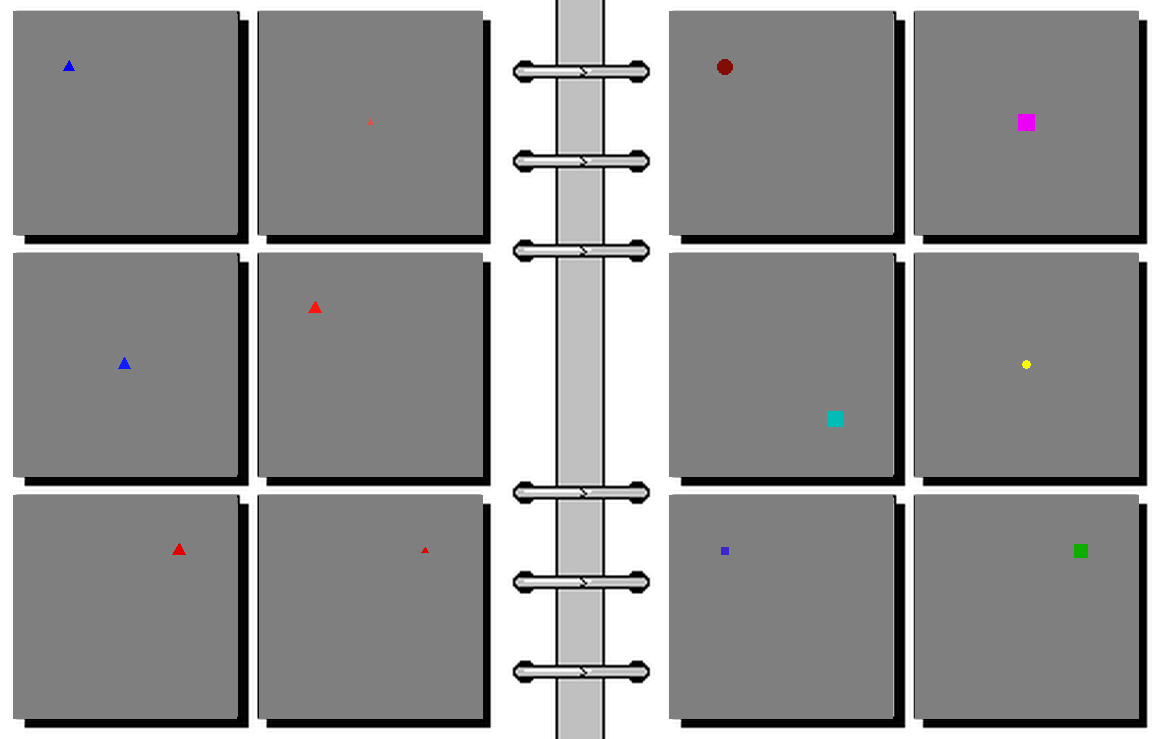
\includegraphics[width=.8\linewidth]{imgs/bongard/easy-0.png}\\
	\begin{dialogue}
		\speak{LLaVA} The image represents a Bongard Problem, which is an abstract visual reasoning task. The problem consists of twelve panels, each containing atomic objects characterized by shape, color, and size. The objects are recursively displaced vertically, horizontally, diagonally, or in a grid pattern.
		
		The panels on the left side of the image all share a single property, which is that the \textcolor{red}{objects are arranged in a grid pattern}. The panels on the right side of the image violate this property, as the objects are not arranged in a grid pattern. This information helps to identify the property that the panels share and the property that the panels on the right side do not share.
		%\\\direct{Did not answer.}
		%\speak{LLaVA} 
		\vspace{1em}
		\speak{MoE-LLaVA} The property that the panels on the left side of the image share is that they all contain objects with the \textcolor{ForestGreen}{same shape} and \textcolor{red}{color}. This property is violated by the panels on the right side, which contain objects with different shapes and colors. The panels on the left side are arranged in a way that they all have the same shape and color, while the panels on the right side have a different arrangement of shapes and colors. This creates a visual pattern that can be analyzed using abstract reasoning and logical operations.
		%\\\direct{Did not answer.}
		%\speak{MoE-LLaVa} 
		\vspace{1em}
		\speak{InternLM-XComposer} Based on the description of the structure and requirements of a Bongard Problem, here is the analysis:
		
		Property Identification: The property shared by each panel in the left half (upper and lower rows) is the presence of \textcolor{red}{both a large triangle and red color}.
		Property Violation in Right Half: Contrarily, the right side has three panels that contradict this property.
		There are instances where there is no triangle present.
		Sometimes there is no red color or it is not accompanied by a large shape.
		Symmetry Comparison: The symmetric aspect (across the central vertical axis) suggests that for each matched pair:
		On both sides, the object should correspond to have small, medium, or large size, but only red triangles should be considered 'large' as per the existing pattern.
		\textcolor{red}{Red should remain the primary color that indicates an object (when it occurs alongside a triangle) is 'large'}.
		Object Characteristics:
		Color Constraints: Objects on the right side must either lack red or \textcolor{ForestGreen}{have shapes other than triangles}.
		Comparative Approach: Analyze patterns across all panels by comparing color and shape occurrences.
		
		Therefore, the property is the relationship between color, shape, and size as follows:
		
		Color + Shape: The pairings indicate specific patterns where certain properties appear together in some panels, not in others.
		
		This analysis reveals the logical constraints based on the given panels.
		%\\\direct{Did not answer.}
		%\speak{InternLM-XComposer} 
	\end{dialogue}
	\captionof{figure}{\textsc{KANDY-Bongard-1},  Task 0: ``A triangle''}
	\label{fig:task0-bongard}
\end{tcolorbox}




\begin{tcolorbox}[breakable,enhanced jigsaw,opacityback=0,]
	\centering
	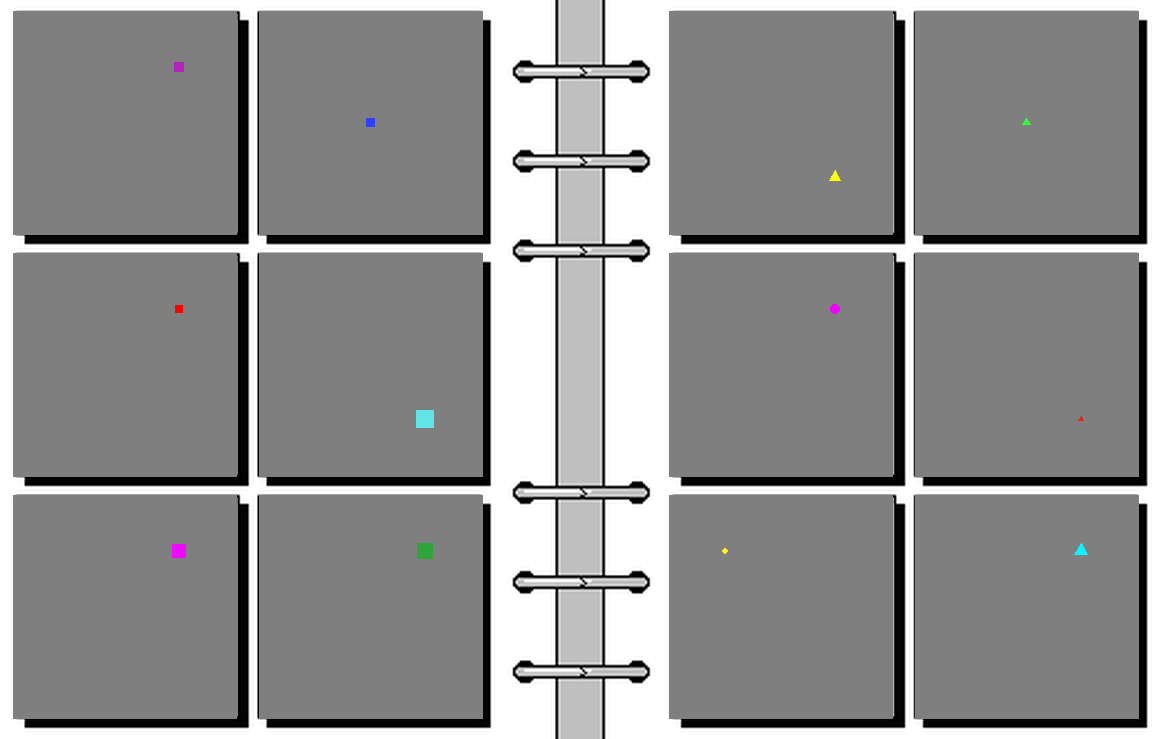
\includegraphics[width=.8\linewidth]{imgs/bongard/easy-1.png}\\
	\begin{dialogue}
		\speak{LLaVA} The image consists of twelve panels, each containing atomic objects characterized by shape, color, and size. The panels on the left side of the image all share a single property, while the panels on the right side violate that property.
		
		To solve this Bongard Problem, we can reason about the spatial relations, patterns, and counting of the objects. Since the panels on the left share a single property, we can deduce that the objects within each panel are arranged in a consistent pattern, such as a grid or a specific arrangement. We can also count the number of objects in each panel to identify any patterns or trends.
		
		For example, if we notice that there are three objects in each panel on the left, we can infer that the property they share is related to the number of objects. Similarly, if we observe that the objects on the right violate the property, we can deduce that the number of objects in each panel is different from the left side.
		
		By analyzing the spatial relations and patterns of the objects, we can identify the property that the panels on the left share and the property that the panels on the right violate. This will help us understand the underlying structure of the image and solve the Bongard Problem.
		\\\direct{Did not answer.}
		\speak{LLaVA} Based on the image, we can observe that the panels on the left share a single property, while the panels on the right violate that property. To solve the Bongard Problem, we need to identify the property and the pattern of the objects within each panel.
		
		First, we can count the number of objects in each panel to identify any patterns or trends. In the left panels, \textcolor{red}{we can see that there are three objects in each panel}. This suggests that the property they share is related to the number of objects.
		
		Next, we can analyze the spatial relations and patterns of the objects within each panel. Since the objects are arranged in a consistent pattern, such as a grid or a specific arrangement, we can deduce that the property they share is related to the arrangement of the objects.
		
		Based on these observations, we can conclude that the property shared by the panels on the left is that they contain \textcolor{red}{three objects} arranged in a specific pattern, while the panels on the right violate this property by having a different number of objects or arrangement.
		
		Therefore, the solution to the Bongard Problem is that the panels on the left share a property related to the number of objects and arrangement, while the panels on the right violate this property.
		\vspace{1em}
		\speak{MoE-LLaVA} The property that the panels on the left side of the image share is that \textcolor{ForestGreen}{they all contain only one type of object}. The property that the panels on the right side violate is that they contain objects of different types. This can be inferred by observing the different shapes, colors, and sizes of the objects in each panel. The panels on the left side are all identical, while the panels on the right side contain \textcolor{ForestGreen}{a mix of shapes, colors, and sizes}. This creates a visual pattern that can be used to solve the Bongard Problem.
		%\\\direct{Did not answer.}
		%\speak{MoE-LLaVa} 
		\vspace{1em}
		\speak{InternLM-XComposer} To solve the Bongard Problem, identify which object property is consistent in the left panels and violated in the right panels.
		
		Based on the visual patterns:
		
		In the left panels (Panels 2-5, 8-11), \textcolor{red}{all objects have a smaller shape relative to at least another element in their panel}.
		The right panels (Panels 1, 6, 12) do not contain this trend; there are no two differently sized shapes related by size comparison within these panels.
		
		Therefore, the property that changes from left to right panels is:
		
		\textcolor{red}{No two objects sharing the smallest or largest shapes (i.e., one object must be definitively smaller/larger than the rest)}.
		
		This helps identify the key feature that is violated across the set.
		%\\\direct{Did not answer.}
		%\speak{InternLM-XComposer} 
	\end{dialogue}
	\captionof{figure}{\textsc{KANDY-Bongard-1},  Task 1: ``A square''}
	\label{fig:task1-bongard}
\end{tcolorbox}




\begin{tcolorbox}[breakable,enhanced jigsaw,opacityback=0,]
	\centering
	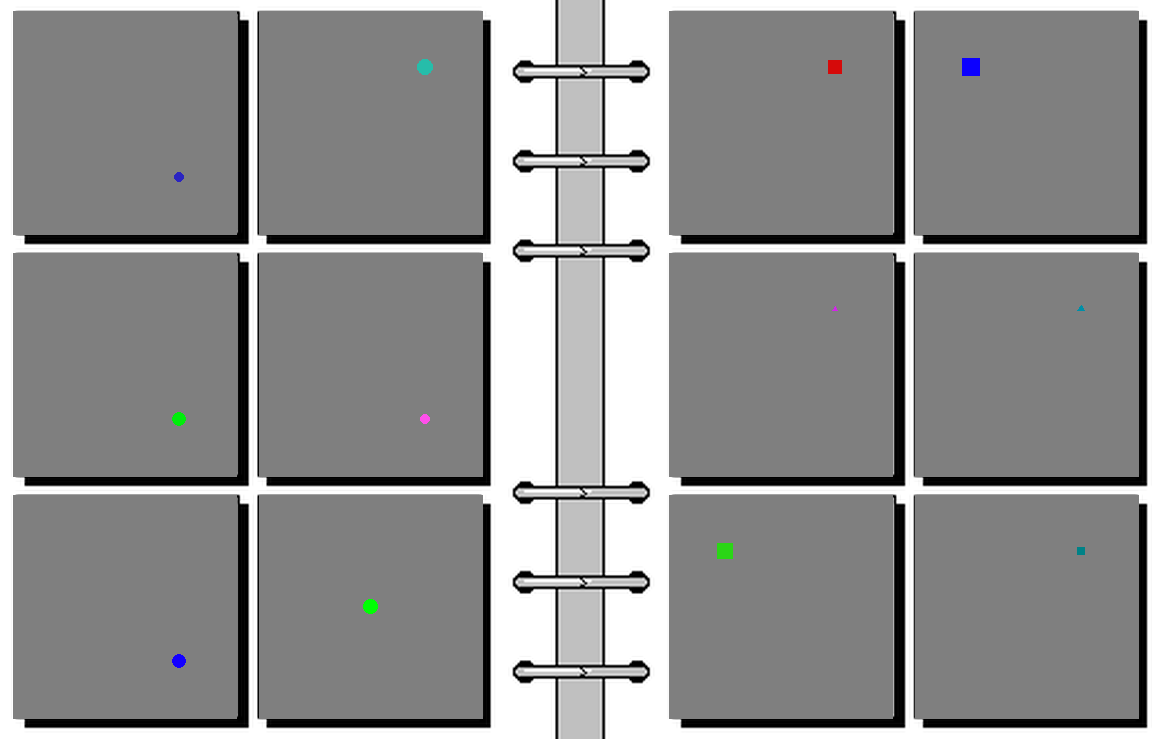
\includegraphics[width=.8\linewidth]{imgs/bongard/easy-2.png}\\
	\begin{dialogue}
		\speak{LLaVA} The image represents a Bongard Problem, which is an abstract visual reasoning task. The problem consists of twelve panels, each containing atomic objects characterized by shape, color, and size. The objects are recursively displaced vertically, horizontally, diagonally, or in a grid pattern.
		
		The panels on the left side of the image all share a single property, which is that \textcolor{red}{the objects are arranged in a grid pattern}. This can be observed by the alignment of the objects within each panel. On the other hand, the panels on the right side of the image violate this property, as the objects are not arranged in a grid pattern. Instead, \textcolor{red}{they are displaced in various directions, such as vertically, horizontally, or diagonally}.
		
		To solve this problem, one needs to identify the specific property that the objects on the left share and then look for the differences in the objects' arrangement on the right side. By doing so, one can determine the property that the objects on the right violate.
		
		\vspace{1em}
		\speak{MoE-LLaVA} The property that the panels on the left side of the image violate is the \textcolor{red}{color of the atomic objects}. All the panels on the left share a single color for the objects, while the panels on the right violate this property by having different colors for the objects. This property violation creates an abstract visual reasoning task, where one needs to identify the pattern and distinguish between the panels on the left and the right.
		%\\\direct{Did not answer.}
		%\speak{MoE-LLaVa} 
		\vspace{1em}
		\speak{InternLM-XComposer} Based on the given image and understanding of Bongard Problems, let's determine the shared property in the panels on the left side and its violation on the right side.
		
		Observing the panels left of the separator:
		
		In each panel, all the shapes have the same size with a uniform distribution of color \textcolor{ForestGreen}{(each panel contains distinct colors)}.
		\textcolor{red}{There is no repetition of shape across adjacent panels (each shape appears only once)}.
		
		On the right side of the separator:
		
		The panel contains a large circle, two small squares, an irregularly sized triangle, and a small magenta diamond. All these objects appear in the rows and do not violate the size property from the left side.
		The two rightmost panels contain small areas of different colored shapes.
		
		Observing both sides carefully, \textcolor{red}{I deduce that there is no violation by shape or color size in the right panels, nor are there consistency issues in arrangement}.
		
		Re-evaluating:
		
		\textcolor{red}{The property should be related to object color, not size}.
		\textcolor{ForestGreen}{The arrangement does not seem to violate a spatial or logical principle either (e.g., arrangement or overlapping)}.
		
		Upon re-evaluating patterns and spatial arrangement more deeply, the key realization comes when noticing the \textcolor{red}{number of shapes per panel and their sizes}:
		
		Both the left and right panels contain small shapes. On the right side, we observe that only three of the rows contain fully visible shapes.
		The pattern here is not about the exact count so much as it is considering what might be implied: if six panels are considered as a sequence of three rows horizontally, this implies a specific alignment pattern.
		
		\textcolor{red}{The left panels show consistent single-row alignments but violate this pattern in the right panels as they contain mixed shapes across two rows}.
		
		The violating feature is thus:
		
		{The panels on the right follow a grid pattern that alternates single-row and double-row distributions}, not consistently sticking to any one format throughout the panel.
		
		By defining these observations clearly through pattern recognition and spatial logic, we identify the inconsistency in the Bongard Problem, specifically regarding the spatial arrangement of objects within the panels.
		%\\\direct{Did not answer.}
		%\speak{InternLM-XComposer} 
	\end{dialogue}
	\captionof{figure}{\textsc{KANDY-Bongard-1},  Task 2: ``A circle''}
	\label{fig:task2-bongard}
\end{tcolorbox}




\begin{tcolorbox}[breakable,enhanced jigsaw,opacityback=0,]
	\centering
	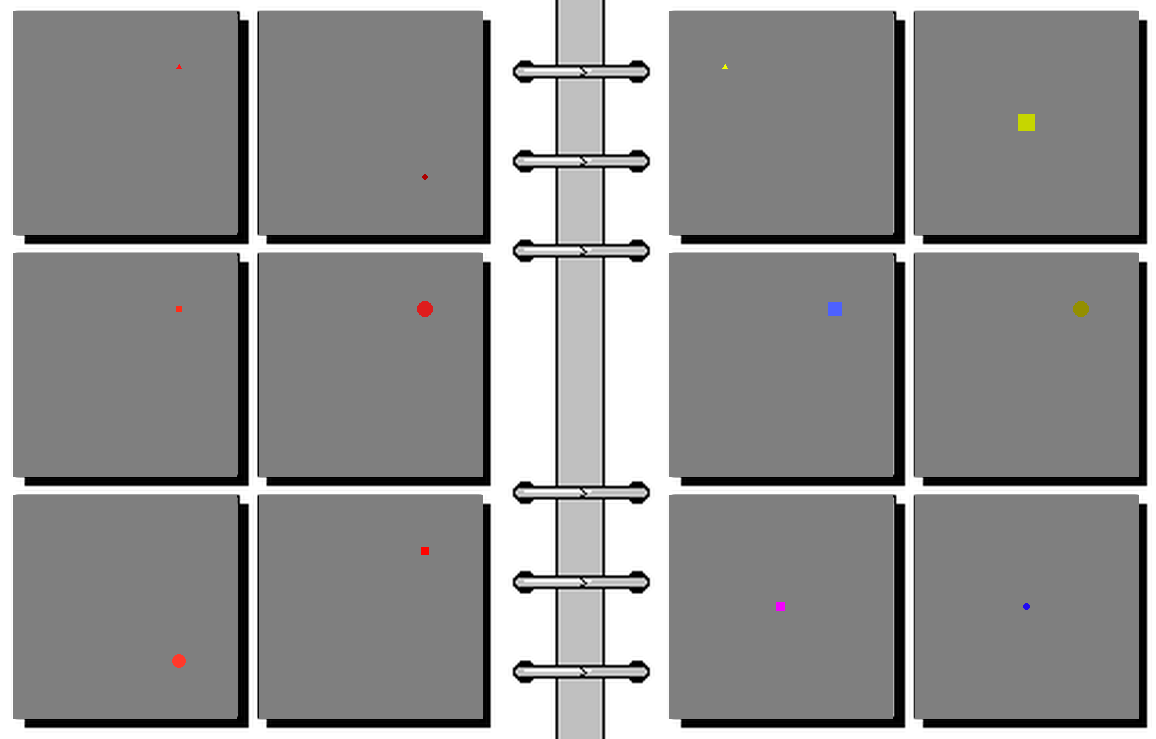
\includegraphics[width=.8\linewidth]{imgs/bongard/easy-3.png}\\
	\begin{dialogue}
		\speak{LLaVA} The image represents a Bongard Problem, which is an abstract visual reasoning task. The problem consists of twelve panels, each containing atomic objects characterized by shape, color, and size. The objects are recursively displaced vertically, horizontally, diagonally, or in a grid pattern.
		
		The panels on the left side of the image all share a single property, which is that \textcolor{red}{the objects are arranged in a grid pattern}. The objects in each panel are positioned in a grid-like arrangement, with each object occupying a specific position within the grid.
		
		On the other hand, the panels on the right side of the image violate this property. The objects in these panels are not arranged in a grid pattern, but rather in a more random or scattered arrangement. This difference in arrangement between the left and right panels helps to distinguish the property that the left panels share.
		%\\\direct{Did not answer.}
		%\speak{LLaVA} 
		\vspace{1em}
		\speak{MoE-LLaVA} The property that the panels on the left side of the image violate is that they all share a single property, which is \textcolor{ForestGreen}{the color of the atomic objects}. The panels on the right side of the image, on the other hand, do not violate any property.
		
		To solve this problem, one can use logical reasoning and pattern recognition. By observing the arrangement of the panels and the properties of the atomic objects within them, one can deduce that the panels on the left share a common color, while the panels on the right do not. This can be further confirmed by analyzing the shapes and sizes of the objects within each panel.
		
		In addition, one can use spatial reasoning to determine the relationships between the panels and the atomic objects within them. By analyzing the patterns and symmetries present in the image, one can deduce the properties of the objects within each panel and the relationships between them.
		
		Overall, the key to solving this problem is to carefully analyze the image and use logical reasoning and pattern recognition to deduce the properties of the atomic objects and the relationships between them.
		%\\\direct{Did not answer.}
		%\speak{MoE-LLaVa} 
		\vspace{1em}
		\speak{InternLM-XComposer} The property depicted involves the pattern of color and position to signify object symmetry or arrangement. Here is the analysis:
		
		\textcolor{ForestGreen}{Red Object Placement: In each panel on the left side, there are red objects} placed symmetrically at the top and bottom corners.
		\textcolor{red}{Yellow Object Placement: On the right side, one of the panels has a single yellow square, which breaks the symmetry by being placed away from the corner position}.
		
		Based on this information, the shared property across all left panels is that they contain \textcolor{ForestGreen}{red objects} \textcolor{red}{in specific positions}, creating symmetry. The right panels violate this symmetry by either having different placement patterns (square instead of two separate circles) or different colors (yellow instead of red).
		%\\\direct{Did not answer.}
		%\speak{InternLM-XComposer} 
	\end{dialogue}
	\captionof{figure}{\textsc{KANDY-Bongard-1},  Task 3: ``A red object''}
	\label{fig:task3-bongard}
\end{tcolorbox}




\begin{tcolorbox}[breakable,enhanced jigsaw,opacityback=0,]
	\centering
	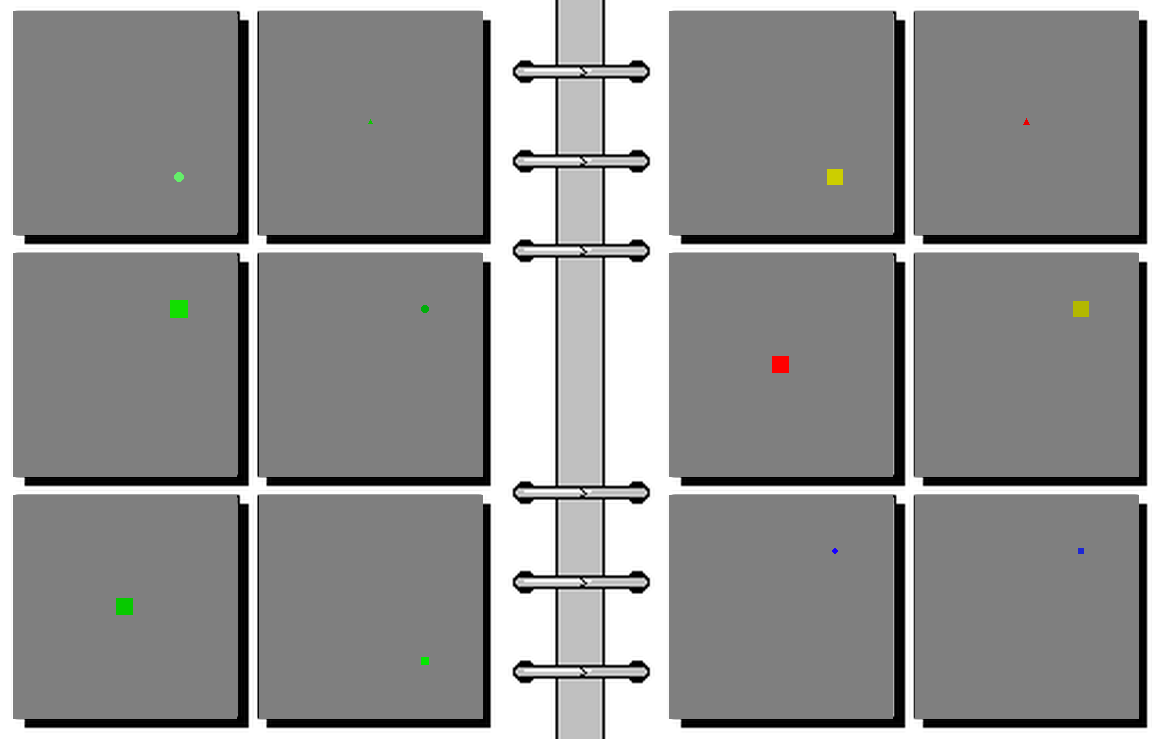
\includegraphics[width=.8\linewidth]{imgs/bongard/easy-4.png}\\
	\begin{dialogue}
		\speak{LLaVA} The image consists of twelve panels, each containing atomic objects characterized by shape, color, and size. The objects are recursively displaced vertically, horizontally, diagonally, or in a grid pattern. The panels on the left side of the image all share a single property, while the panels on the right side violate that property.
		
		To solve this Bongard Problem, one can reason about the spatial relations, patterns, and counting of the objects. The objects are arranged in a grid pattern, which suggests that they might be organized in a systematic manner. By counting the number of objects in each panel, one can identify the property that the left panels share. For example, if there are three objects in each panel, the left panels might share the property of having three objects.
		
		Additionally, one can reason about the logical operators and symmetries to identify the property. For instance, if the left panels all have three objects, the right panels might have a different number of objects, such as four or five. By comparing the number of objects in each panel, one can identify the property that the left panels share and the property that the right panels violate.
		\\\direct{Did not answer.}
		\speak{LLaVA} To solve the Bongard Problem, we can reason about the spatial relations, patterns, and counting of the objects. The objects are arranged in a grid pattern, which suggests that they might be organized in a systematic manner. By counting the number of objects in each panel, we can identify the property that the left panels share.
		
		In this case, \textcolor{red}{there are three objects in each panel on the left side}. The left panels all share the property of having three objects. On the right side, the panels violate this property, which means that they have a different number of objects.
		
		To determine the property that the right panels violate, we can count the number of objects in each panel on the right side. If there are three objects in each panel, the right panels might share the property of having three objects. However, since the left panels all have three objects, the right panels must have a different number of objects.
		
		Therefore, the right panels violate the property of having three objects, which means that \textcolor{red}{they have either four or five objects in each panel}. By identifying the property that the left panels share and the property that the right panels violate, we have successfully solved the Bongard Problem.
		\vspace{1em}
		\speak{MoE-LLaVA} The property that is violated by the panels on the right side of the image is the \textcolor{ForestGreen}{color} of the objects. \textcolor{ForestGreen}{All the objects in the left panels have the same color}, while the objects in the right panels have different colors. This creates a visual contrast between the two sets of panels, making it easier to identify the pattern and solve the Bongard Problem.
		%\\\direct{Did not answer.}
		%\speak{MoE-LLaVa} 
		\vspace{1em}
		\speak{InternLM-XComposer} Observing the image, we can identify that each panel either contains a green dot or an object colored differently. On the left side, \textcolor{ForestGreen}{every panel has at least one green dot in it}.
		
		On the right side of the image:
		
		The first and third panels contain yellow squares instead of dots.
		The second panel on the right side contains a yellow square which is blue in color but located outside the standard position typically occupied by a color dot (like green).
		The fourth panel contains two small squares, a red one and a blue one, both located vertically.
		
		The correct answer is all panels on the left have a color dot property followed by those on the right side violating this property; specifically, only green dots are present on the left and squares fill their places on the right side.
		
		Therefore, ignoring empty panels, \textcolor{ForestGreen}{the feature to look for is whether a panel contains a green dot} or \textcolor{ForestGreen}{a square colored differently – the latter being the characteristic of the right side's panels}.
		%\\\direct{Did not answer.}
		%\speak{InternLM-XComposer} 
	\end{dialogue}
	\captionof{figure}{\textsc{KANDY-Bongard-1},  Task 4: ``A green object''}
	\label{fig:task4-bongard}
\end{tcolorbox}




\begin{tcolorbox}[breakable,enhanced jigsaw,opacityback=0,]
	\centering
	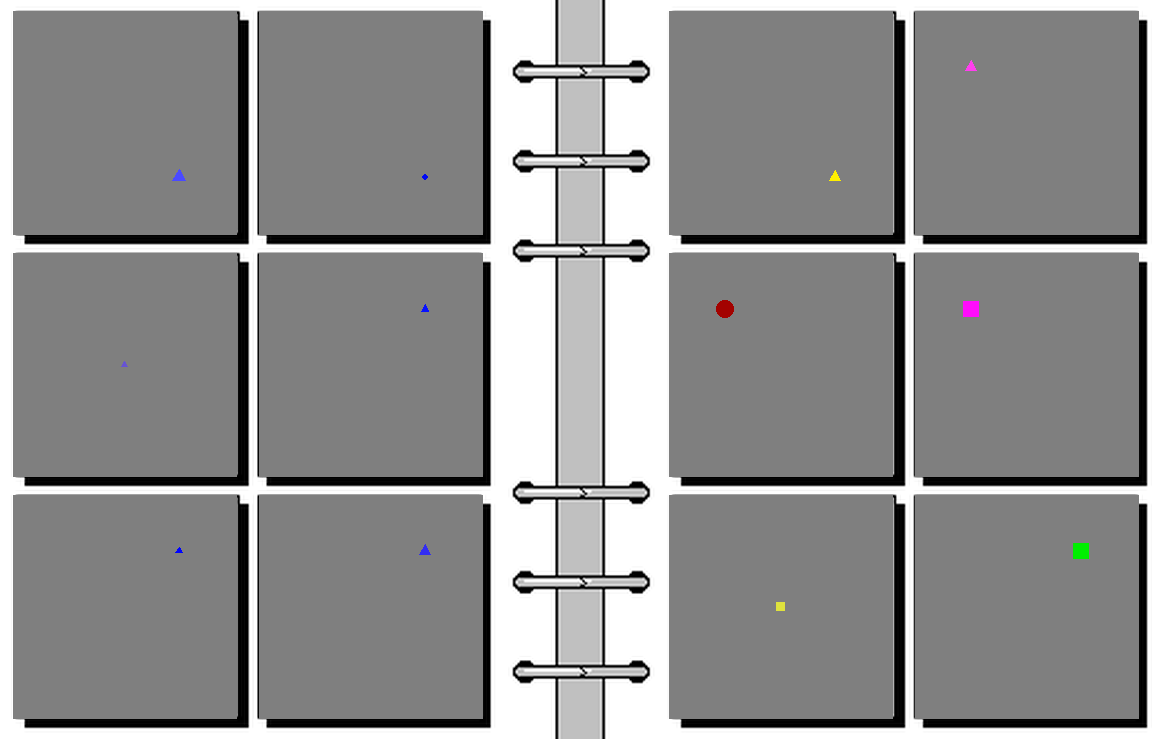
\includegraphics[width=.8\linewidth]{imgs/bongard/easy-5.png}\\
	\begin{dialogue}
		\speak{LLaVA} The image represents a Bongard Problem, which is an abstract visual reasoning task. The problem consists of twelve panels, each containing atomic objects characterized by shape, color, and size. The objects are recursively displaced vertically, horizontally, diagonally, or in a grid pattern.
		
		The panels on the left side of the image all share a single property, which is that \textcolor{red}{the objects are arranged in a grid pattern}. This can be observed by the alignment of the objects within each panel. On the other hand, the panels on the right side of the image violate this property, as the objects are not arranged in a grid pattern. Instead, they are placed in a more random or scattered arrangement.
		
		To solve this problem, one would need to identify the specific property that the objects on the left share and then determine how it differs from the objects on the right. By doing so, one can deduce the rule that governs the arrangement of the objects in the image.
		%\\\direct{Did not answer.}
		%\speak{LLaVA} 
		\vspace{1em}
		\speak{MoE-LLaVA} The property that the panels on the left side of the image share is that \textcolor{red}{they all contain the same shape, color, and size of the atomic objects}. This property is violated by the panels on the right side, which contain different shapes, colors, and sizes of the atomic objects. The panels on the right side also violate the property of having the same shape, color, and size of the atomic objects. This property is important in the Bongard Problem, as it helps to identify the patterns and relationships between the different panels.
		%\\\direct{Did not answer.}
		%\speak{MoE-LLaVa} 
		\vspace{1em}
		\speak{InternLM-XComposer} The panels on the left side all have \textcolor{ForestGreen}{smaller colored objects}, while these properties are violated in the right panels. This means that for a given panel to be considered as having only the smaller objects, all small objects of a specific color must align vertically and/or horizontally with each other, without any additional colors or larger sizes interfering.
		
		The pattern observed is:
		
		Each column on the left side has triangular blue objects that form a vertical alignment.
		The columns \textcolor{red}{do not exhibit the same color or shape repeatedly}.
		Each individual column within the left side features at least one set of small objects arranged either in a vertical or horizontal sequence.
		
		On the right side, at some point, the patterns of these sequences are disrupted by introducing non-matching or mismatched object types or sizes that differ from the single-color, small size property seen in the left side panels.
		
		The key feature used here:
		
		All patterns follow the condition that small objects maintain consistency in their appearance (\textcolor{ForestGreen}{same color} and same size).
		
		The logical operators that help determine the correct property are:
		
		Disjunctions ($\vee$), to include the presence of any small object of the specific color
		Negations ($\neg$), to indicate the absence of large and other colors
		Conjunctions ($\wedge$), to require a series of small-colored objects
		
		Therefore, the correct answer should be "\textcolor{red}{Each pattern must show a vertical or horizontal sequence where all objects are small}, \textcolor{ForestGreen}{using the same color}."
		%\\\direct{Did not answer.}
		%\speak{InternLM-XComposer} 
	\end{dialogue}
	\captionof{figure}{\textsc{KANDY-Bongard-1},  Task 5: ``A blue object''}
	\label{fig:task5-bongard}
\end{tcolorbox}




\begin{tcolorbox}[breakable,enhanced jigsaw,opacityback=0,]
	\centering
	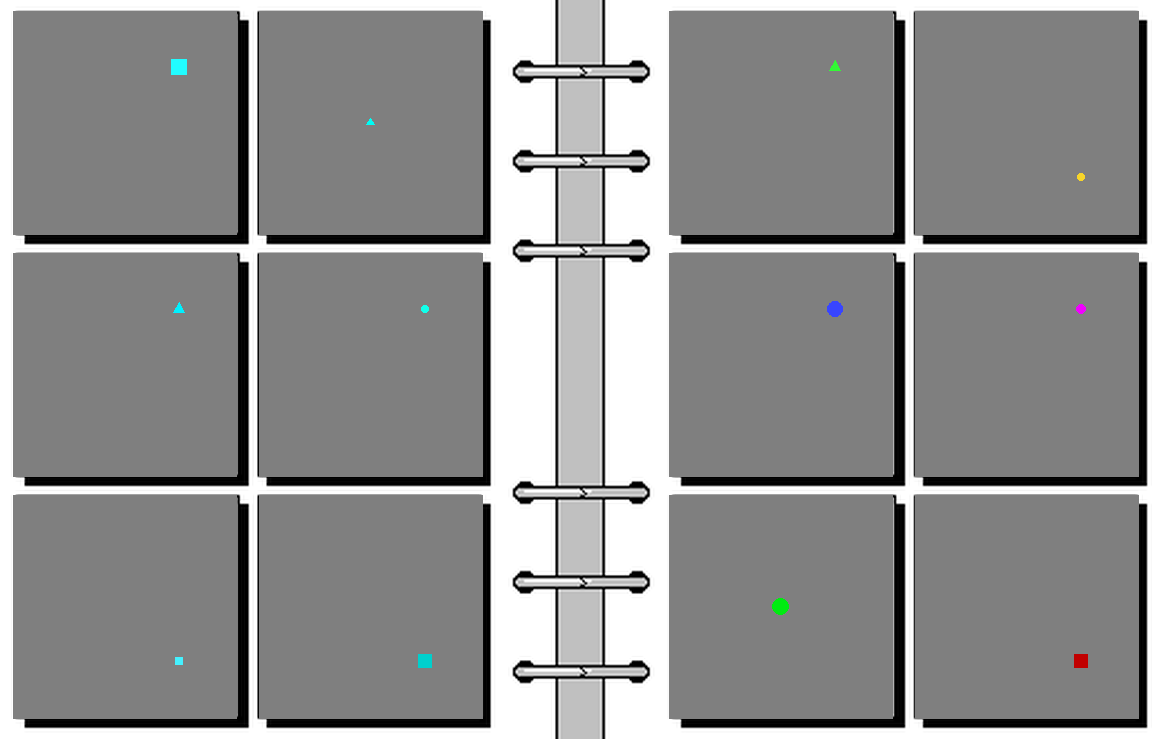
\includegraphics[width=.8\linewidth]{imgs/bongard/easy-6.png}\\
	\begin{dialogue}
		\speak{LLaVA} The image represents a Bongard Problem, which is an abstract visual reasoning task. The task consists of twelve panels, each containing atomic objects characterized by shape, color, and size. The objects are recursively displaced vertically, horizontally, diagonally, or in a grid pattern.
		
		In this particular image, the panels on the left side all share a single property, while the panels on the right side violate that property. The property in question is that \textcolor{red}{all the objects in the left panels are either triangles or squares}, and \textcolor{red}{they are all green or blue in color}. In contrast, the objects in the right panels are a mix of triangles, squares, and circles, and they come in various colors.
		
		To solve this problem, one would need to analyze the spatial relationships and patterns within the panels, as well as the properties of the objects themselves. By identifying the common property among the left panels and the violation of that property in the right panels, one can deduce the correct answer to the Bongard Problem.
		%\\\direct{Did not answer.}
		%\speak{LLaVA} 
		\vspace{1em}
		\speak{MoE-LLaVA} The property that the panels on the right side of the image violate is the color of the atomic objects. All the panels on the left side of the image have \textcolor{ForestGreen}{objects with the same color}, while the panels on the right side have objects with different colors. This property violation creates a visual pattern that can be used to solve the Bongard Problem.
		%\\\direct{Did not answer.}
		%\speak{MoE-LLaVa} 
		\vspace{1em}
		\speak{InternLM-XComposer} To describe the property:
		
		All panels on the left side contain a \textcolor{ForestGreen}{cyan} \textcolor{red}{triangle}, while all panels on the right side display:
		The absence of a cyan triangle (violates the property).
		Objects are smaller in size compared to their corresponding objects on the left side.
		
		Ignoring empty panels and any other possible changes, consider the overall symmetry:
		Panels 1, 6, 7, 12 contain green triangles below cyan squares.
		Panels 2, 3, 4 may have triangles located at the very bottom or within square elements.
		Panels 5, 8, 9 contain blue triangles underneath small yellow circles.
		Panels 10 has two magenta objects near each other.
		
		The shared property among panels on the left is having \textcolor{ForestGreen}{cyan} \textcolor{red}{triangles positioned above or below large colored shapes}, which corresponds with specific color patterns on the given set of atomic objects.
		
		The symmetry can be further examined in terms of the arrangement of larger colored shapes and smaller objects below them (triangles, circles, or squares), ensuring that similar colors follow the same arrangement pattern across the left panels.
		
		%\\\direct{Did not answer.}
		%\speak{InternLM-XComposer} 
	\end{dialogue}
	\captionof{figure}{\textsc{KANDY-Bongard-1},  Task 6: ``A cyan object''}
	\label{fig:task6-bongard}
\end{tcolorbox}




\begin{tcolorbox}[breakable,enhanced jigsaw,opacityback=0,]
	\centering
	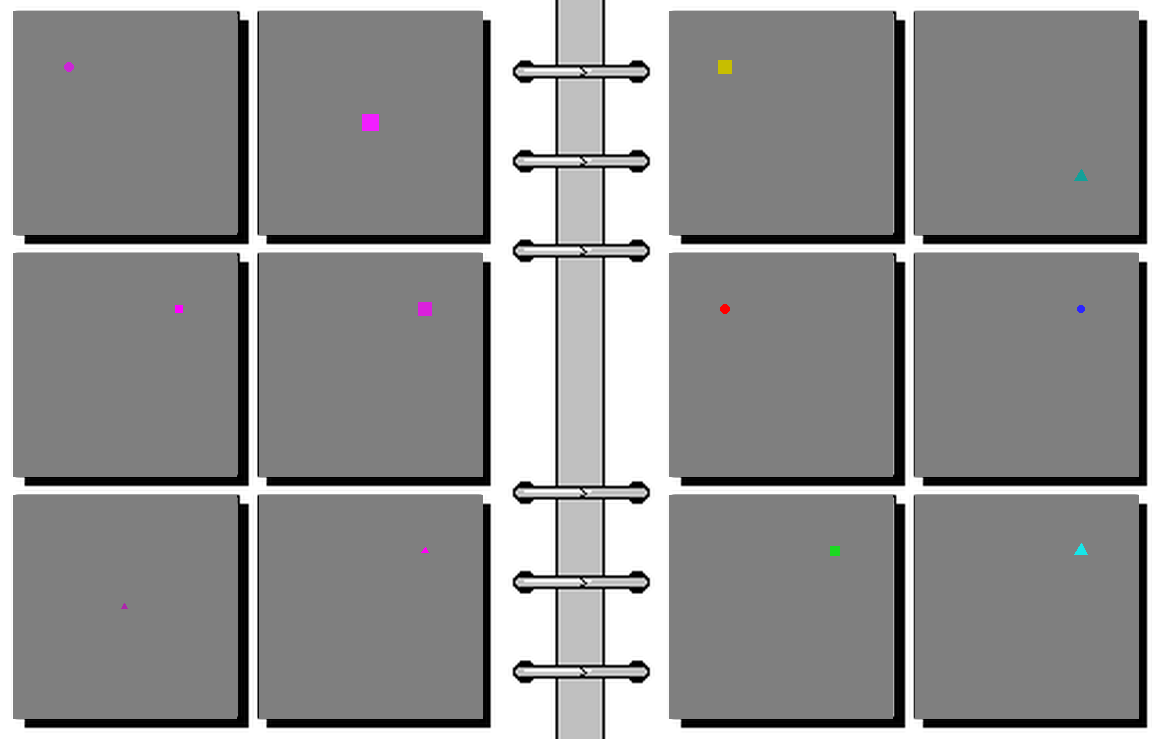
\includegraphics[width=.8\linewidth]{imgs/bongard/easy-7.png}\\
	\begin{dialogue}
		\speak{LLaVA} The image consists of twelve panels, each containing atomic objects characterized by shape, color, and size. The objects are recursively displaced vertically, horizontally, diagonally, or in a grid pattern. The panels on the left side of the image all share a single property, while the panels on the right side violate that property.
		
		To solve this Bongard Problem, we can reason about the spatial relations, patterns, and counting of the objects. Since the objects are recursively displaced, we can expect to see a pattern in their arrangement. The panels on the left side share a single property, which could be related to the shape, color, or size of the objects. For example, all objects in these panels might be \textcolor{red}{triangles} of the \textcolor{ForestGreen}{same color}.
		
		To identify the property, we can count the number of objects in each panel and look for any patterns or similarities. We can also examine the spatial relations between the objects, such as their position relative to each other or the edges of the panels. By combining these observations, we can deduce the property that unifies the objects in the left panels and identify the property that distinguishes them from the objects in the right panels.
		%\\\direct{Did not answer.}
		%\speak{LLaVA} 
		\vspace{1em}
		\speak{MoE-LLaVA} The property that the panels on the left side of the image share is that they all contain only one type of object. The other panels on the right side violate this property by containing multiple types of objects. This property can be inferred by observing the different shapes, colors, and sizes of the objects in each panel. \textcolor{red}{The panels on the left side are all identical}, while the panels on the right side have a variety of objects with different shapes, colors, and sizes. This property can be used to solve the Bongard Problem by identifying the pattern and reasoning about the spatial relationships between the objects in each panel.
		%\\\direct{Did not answer.}
		%\speak{MoE-LLaVa} 
		\vspace{1em}
		\speak{InternLM-XComposer} The property in question is likely related to the arrangement or placement of objects. From the given context:
		
		Panels 1, 3, 7 and 8 contain \textcolor{ForestGreen}{magenta-colored} rectangular objects.
		All these panels are located on the left side.
		
		The consistent feature among these four panels is that each one contains a single, large object.
		
		The "non-property" seen in panel 10, the right side, is an object placed where there would be an absence if following the observed pattern (since four panels share the feature of having exactly one large rectangular object). Therefore, panels on the right side do not have an atomic object.
		
		Continuing down the columns from the right side, panels 11 and 12 seem to follow the property by featuring small objects. But panels 5, 6, and 9 violate this rule by containing no objects at all.
		
		Overall, the established property is that all objects in a particular column are arranged to be either aligned on the diagonal or absent. Therefore, focusing on spatial arrangements and considering patterns:
		
		Property: columns with either alignment or absence of objects based on the grid pattern
		Panels with the property: 1, 3, 7, 8
		Panels violating the property: 1 (although it has a magenta square, it's not vertically aligned with another object)
		Violation on the right side: panels 10, 11, 12, 5, 6, 9
		\\\direct{Exceeded maximum number of tokens.}
		%\\\direct{Did not answer.}
		%\speak{InternLM-XComposer} 
	\end{dialogue}
	\captionof{figure}{\textsc{KANDY-Bongard-1},  Task 7: ``A magenta object''}
	\label{fig:task7-bongard}
\end{tcolorbox}




\begin{tcolorbox}[breakable,enhanced jigsaw,opacityback=0,]
	\centering
	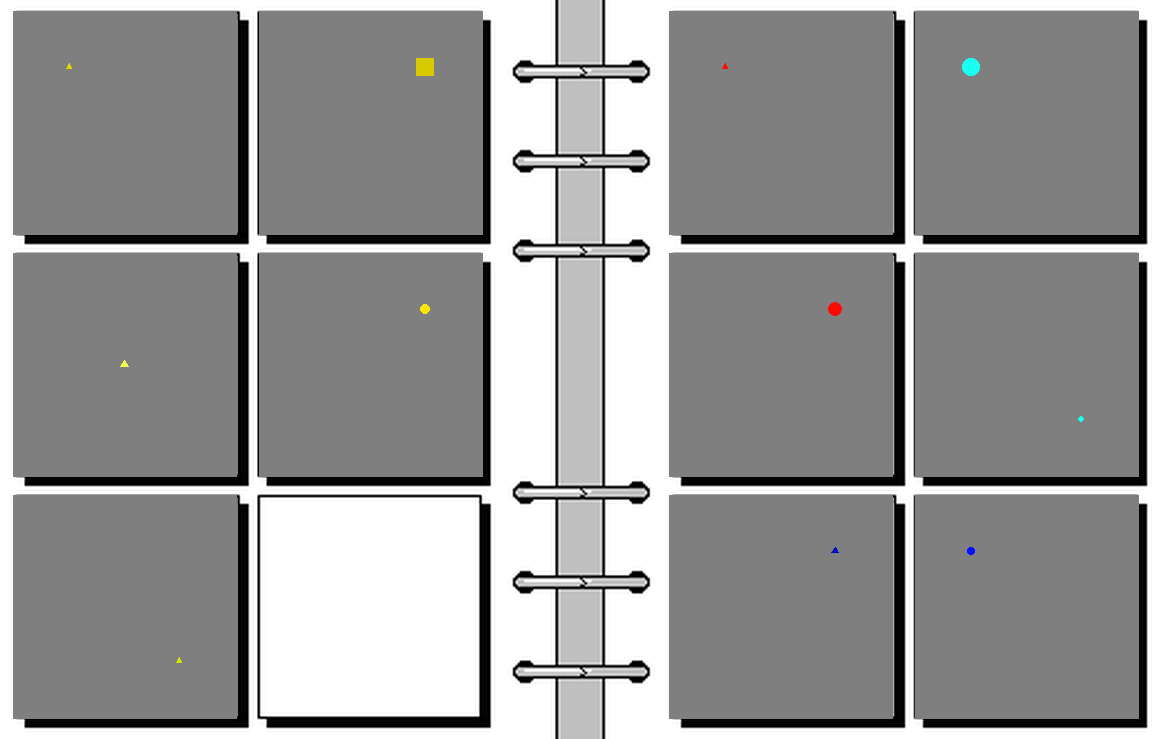
\includegraphics[width=.8\linewidth]{imgs/bongard/easy-8.png}\\
	\begin{dialogue}
		\speak{LLaVA} The image consists of twelve panels, each containing atomic objects characterized by shape, color, and size. The objects are recursively displaced vertically, horizontally, diagonally, or in a grid pattern. The panels on the left side of the image all share a single property, while the panels on the right side violate that property.
		
		The property that the panels on the left share is that all the objects are of the \textcolor{ForestGreen}{same color}, which is \textcolor{red}{blue}. This can be inferred by observing the objects in the panels and noticing that they all have the same color. The panels on the right side, on the other hand, have objects with different colors, which violates the property shared by the panels on the left.
		%\\\direct{Did not answer.}
		%\speak{LLaVA} 
		\vspace{1em}
		\speak{MoE-LLaVA} The property that the panels on the left side of the image share is that they all contain only one type of object, which is a \textcolor{red}{circle}. The other panels on the right side of the image violate this property by containing multiple types of objects, including squares, triangles, and circles. This property can be used to reason about the spatial relations between the objects in each panel and to identify patterns and symmetries within the image. For example, one could count the number of circles in each panel and compare them to the number of squares and triangles to determine if there is a consistent pattern. Additionally, one could use logical operators to determine if the objects in each panel are arranged in a grid pattern or if they are randomly placed.
		%\\\direct{Did not answer.}
		%\speak{MoE-LLaVa} 
		\vspace{1em}
		\speak{InternLM-XComposer} The image depicts a Bongard Problem. The left side of the image shows images with properties that are consistent across all panels, while the right side contains images that violate this property.
		
		By analyzing the patterns and relationships between the objects in each panel, we can identify the key feature being violated:
		
		Panel Structure: All panels have three atomic objects (i.e., shapes).
		
		Object Properties:
		In certain panels, the largest shape (based on area) is red.
		Some panels contain at least one magenta or cyan-colored triangle.
		All panels containing magenta or cyan triangles have small yellow squares on top.
		
		Violation on Right: The panels on the right side deviate from the pattern seen on the left. They include objects where these strict relationships do not hold true.
		
		Based on the given information:
		
		One characteristic observed among the panels on the left is related to symmetry and color. \textcolor{red}{A common attribute for some panels is the presence of both a large red shape and a small colored triangle or square on top}.
		
		The panels on the right violate this specific attribute because they contain either an object with incorrect colors or sizes, disregarding the red shape requirement.
		
		Final Description:
		
		The left panels have \textcolor{red}{at least one large red shape and a small yellow or magenta/triangle or cyan/square positioned on top of it}. The right panels violate this by either having a different color or size, or not having a similar small shape on top.
		
		Ensuring the logical consistency of this pattern, the unique feature that determines whether a panel follows the property is \textcolor{red}{the presence of a small yellow or magenta/triangle above the larger object}, ensuring \textcolor{ForestGreen}{that the color (yellow or }\textcolor{red}{magenta}\textcolor{ForestGreen}{) is constant in the left panels} but absent or varied in the right panels.
		%\\\direct{Did not answer.}
		%\speak{InternLM-XComposer} 
	\end{dialogue}
	\captionof{figure}{\textsc{KANDY-Bongard-1},  Task 8: ``A yellow object''}
	\label{fig:task8-bongard}
\end{tcolorbox}




\begin{tcolorbox}[breakable,enhanced jigsaw,opacityback=0,]
	\centering
	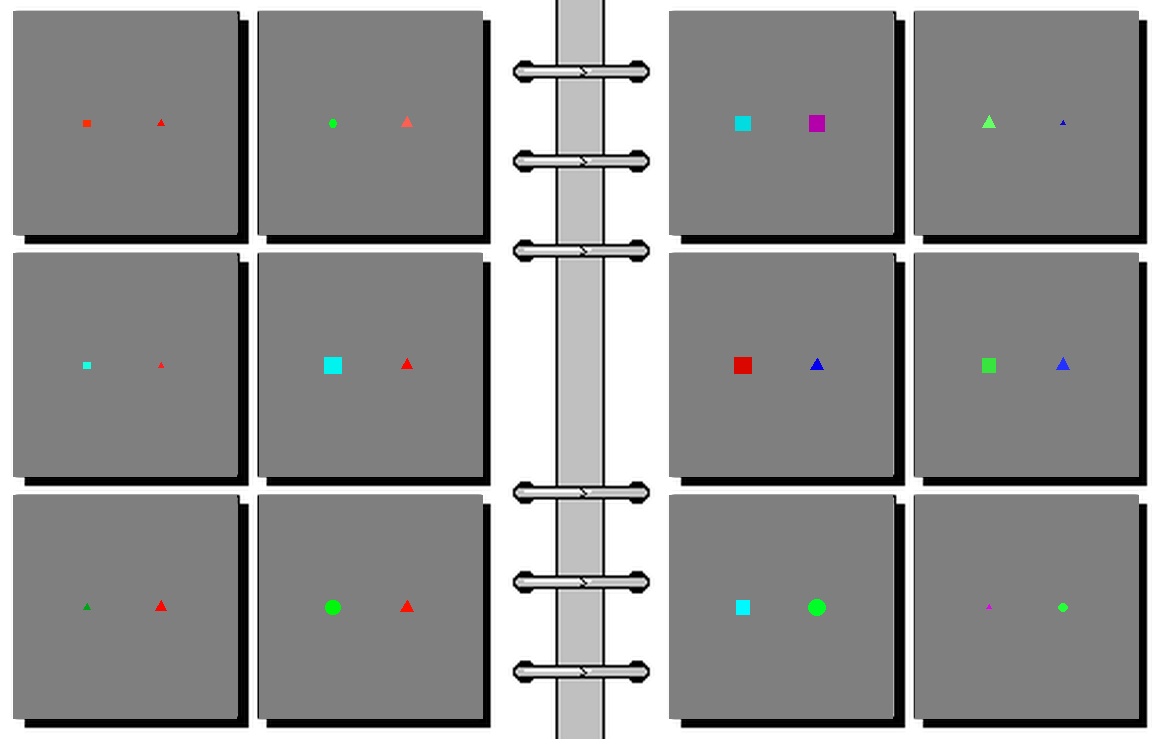
\includegraphics[width=.8\linewidth]{imgs/bongard/easy-9.png}\\
	\begin{dialogue}
		\speak{LLaVA} The image features twelve panels, each containing atomic objects characterized by shape, color, and size. The objects are recursively displaced vertically, horizontally, diagonally, or in a grid pattern. The panels on the left side of the image all share a single property, while the panels on the right side violate that property.
		
		To solve this Bongard Problem, one can reason about the spatial relations, patterns, and counting of the objects. The objects are arranged in a grid pattern, and each panel contains a specific number of objects. By examining the arrangement and counting the objects, one can identify the property that the panels on the left share. Additionally, by comparing the panels on the left and right, one can determine the property that the panels on the right violate.
		
		To further narrow down the possible properties, one can consider the shapes, colors, and sizes of the objects. For example, if all objects are triangles, the property could be related to the shape. If all objects are green, the property could be related to the color. By examining the spatial relations and patterns of the objects, one can identify the property that unifies the panels on the left and differentiates them from the panels on the right.
		\\\direct{Did not answer.}
		\speak{LLaVA} After analyzing the image, it appears that \textcolor{red}{the atomic objects are arranged in a grid pattern}, with each panel containing a specific number of objects. The objects within each panel can be characterized by some property. The panels on the left part of the image all share a single property, while the panels on the right side violate that property.
		
		Upon closer examination, it can be observed that all objects in the left panels are \textcolor{ForestGreen}{triangles with a specific color}, while the objects in the right panels are squares with a different color. The property that unifies the panels on the left is the shape of the objects, which are all triangles. The property that differentiates the panels on the right is the color of the objects, which is different from the color of the objects in the left panels.
		
		In summary, the left panels share the property of \textcolor{ForestGreen}{having triangular objects with a specific color}, while the right panels violate this property by having square objects with a different color.
		\vspace{1em}
		\speak{MoE-LLaVA} The property that the panels on the right side of the image violate is the \textcolor{red}{color of the atomic objects}. All the panels on the left side of the image have objects with the same color, while the panels on the right side have objects with different colors. This difference in color is the main distinguishing feature between the two sets of panels.
		%\\\direct{Did not answer.}
		%\speak{MoE-LLaVa} 
		\vspace{1em}
		\speak{InternLM-XComposer} The panels have two distinct color arrangements.
		
		Property: \textcolor{red}{The upper halves of the images on the left need to follow a color grid pattern where each column follows another}. For instance, there are three columns in each panel.
		
		Violation: The same property does not apply to the lower halves.
		
		Let's work through this:
		
		All panels (ignoring any empty ones) contain 6 shapes and colors (2 triangles, 2 squares/blocks, and either 2 circles or 2 of one specific color circle).
		The first two columns form a 1x2 square (a horizontal arrangement where the blue circle is in row 1 and the large triangle is in row 3). The third column has a unique shape/color that differs from these two columns.
		
		Therefore, considering spatial relations and arrangement of objects, identify that for a consistent layout, similar color patterns should hold true but not in a grid pattern where each column is similar.
		%\\\direct{Did not answer.}
		%\speak{InternLM-XComposer} 
	\end{dialogue}
	\captionof{figure}{\textsc{KANDY-Bongard-1},  Task 9: ``There is a red triangle on the right (two objects)''}
	\label{fig:task9-bongard}
\end{tcolorbox}




\begin{tcolorbox}[breakable,enhanced jigsaw,opacityback=0,]
	\centering
	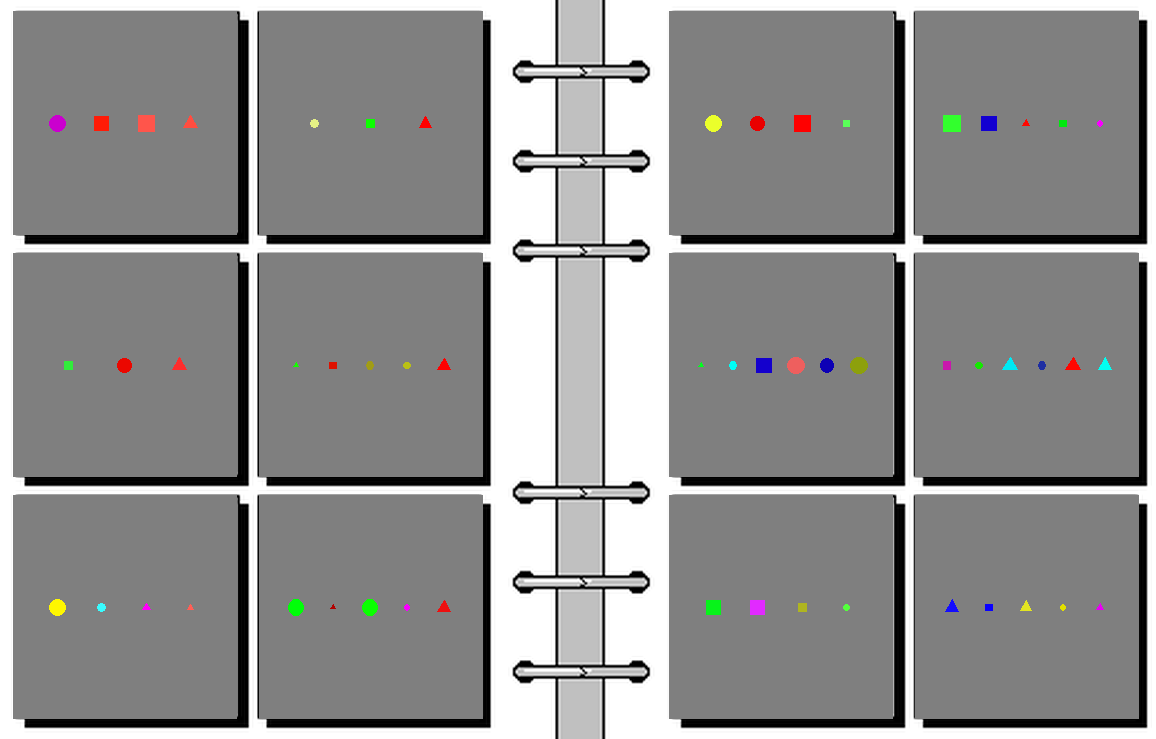
\includegraphics[width=.8\linewidth]{imgs/bongard/easy-10.png}\\
	\begin{dialogue}
		\speak{LLaVA} The image features twelve panels, each containing atomic objects characterized by shape, color, and size. The objects are recursively displaced vertically, horizontally, diagonally, or in a grid pattern. The panels on the left side of the image share a single property, while the panels on the right side violate that property.
		
		To solve this Bongard Problem, one can reason about the spatial relations, patterns, and counting of the objects. The objects are arranged in a grid pattern, which suggests that they might be organized in a systematic manner. By counting the objects in each panel, one can identify the property that the left panels share. For example, if there are three objects in each panel, the left panels might share the property of having three objects.
		
		Additionally, one can reason about the logical operators and symmetries to identify the property. For instance, if the left panels have three objects, the right panels might have a different number of objects, such as four or five. By examining the spatial relations between the objects and their colors, one can further narrow down the property.
		
		In conclusion, the property shared by the left panels is that \textcolor{red}{they all have three objects}, while the right panels violate this property. The objects are arranged in a grid pattern, and their colors and shapes can be used to reason about the property.
		%\\\direct{Did not answer.}
		%\speak{LLaVA} 
		\vspace{1em}
		\speak{MoE-LLaVA} The image represents an abstract visual reasoning task, known as a Bongard Problem, and it is composed of twelve panels. Each panel contains atomic objects characterized by shape ("triangle", "square", "circle"), color ("red", "green", "blue", "cyan", "magenta", "yellow") and size ("small", "large"). Atomic objects are recursively displaced vertically, horizontally, diagonally or in a grid pattern. Objects within each panel can be characterized by some property. The panels on the left part of the image all share a single property. Conversely, the panels on the right side violate that property. Please describe the property, ignoring empty panels, if any. You are allowed to reason in terms of: object properties, spatial relations, patterns, counting, symmetries and logical operators. Enumerate any feature which may help.
		
		The property that the panels on the left side of the image share is that \textcolor{red}{all the objects within them are of the same shape}. The panels on the right side of the image violate this property, as they contain objects of different shapes. This property can be inferred by observing the arrangement of the objects within each panel and comparing them to the other panels. The presence of different shapes in the right side panels indicates that they do not follow the same pattern as the left side panels.
		%\\\direct{Did not answer.}
		%\speak{MoE-LLaVa} 
		\vspace{1em}
		\speak{InternLM-XComposer} Based on the descriptions of the Bongard Problem panels, here are the properties observed:
		
		Horizontal Symmetry: \textcolor{red}{Panels on the left half exhibit horizontal symmetry due to the arrangement of objects and their reflection}.
		Uniformity in Color: \textcolor{red}{The color of all atomic objects remains consistent within each panel}.
		Vertical Displacement: \textcolor{red}{Objects show vertical displacement across the panels}.
		Pattern Repetition: \textcolor{red}{There appears to be a periodic repetition in the object configurations}: triangular, circular, square, then two smaller variations (possibly different shapes or colors).
		
		Identifying a specific property consistent with the description suggests that in all panels on the left side of the image, the atomic objects maintain a uniform position relative to another object within the panel. Specifically, \textcolor{red}{there seems to be a pattern where either three or four objects have the same color across these panels}.
		
		On the right side of the image, there is a disruption in this consistency. Each panel on the right side contains at least one additional color or changes in spatial configuration not seen in the corresponding panels on the left side.
		
		Based on logical reasoning and the layout's structure, the consistent property on the left side is related to the spatial arrangement of these two sets of atomic objects—one set having three of the same color and potentially one large object, the other with four atomic objects all of the same colors as well—where they match in both alignment and color.
		
		The inconsistency on the right side is likely indicated by panels where such an object placement does not align or there’s an additional change that disrupts that uniformity. It suggests elements are not aligned horizontally in a regular pattern, which can be considered the single property that differs across the right set of panels.
		
		Thus, the consistent property among the left side panels involves \textcolor{red}{maintaining a uniform horizontal alignment possibly concerning both the larger and smaller objects' alignment in color and shape}. These observations suggest that the panels break down when such uniformity is compromised, showing variability with respect to object position and color.
		%\\\direct{Did not answer.}
		%\speak{InternLM-XComposer} 
	\end{dialogue}
	\captionof{figure}{\textsc{KANDY-Bongard-1},  Task 10: ``There is a red triangle on the right (many objects)''}
	\label{fig:task10-bongard}
\end{tcolorbox}




\begin{tcolorbox}[breakable,enhanced jigsaw,opacityback=0,]
	\centering
	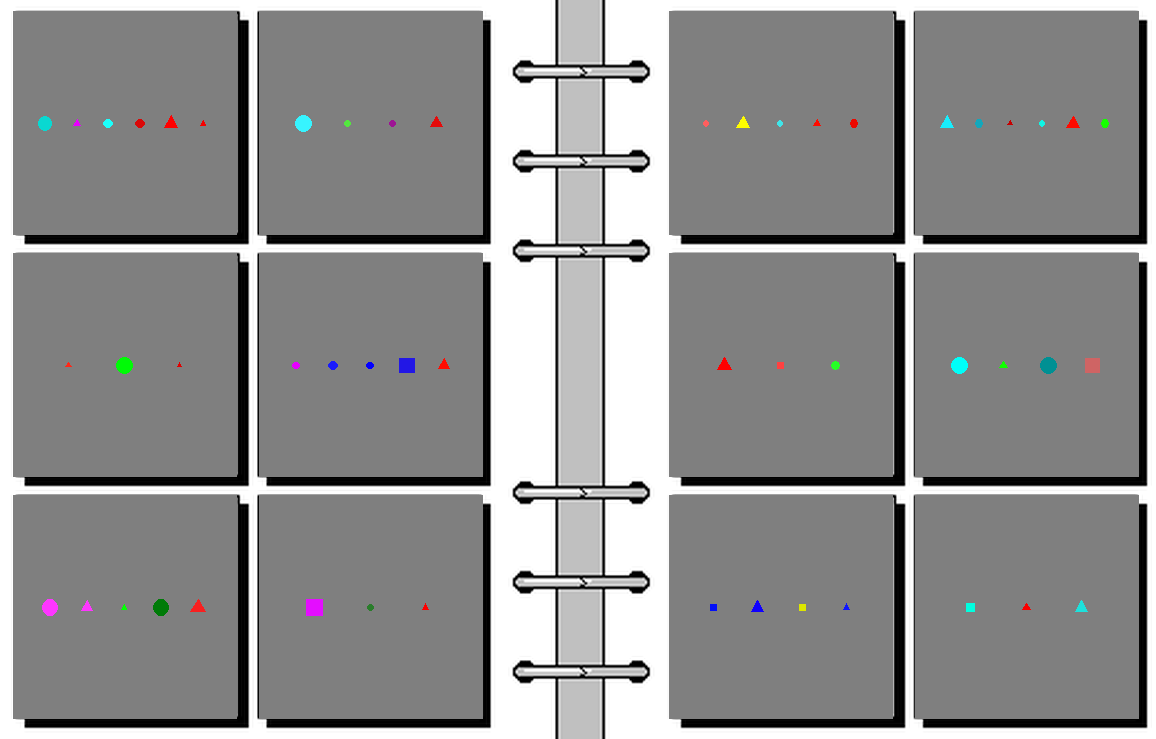
\includegraphics[width=.8\linewidth]{imgs/bongard/easy-11.png}\\
	\begin{dialogue}
		\speak{LLaVA} The image features twelve panels, each containing atomic objects characterized by shape, color, and size. The objects are recursively displaced vertically, horizontally, diagonally, or in a grid pattern. The panels on the left side of the image all share a single property, while the panels on the right side violate that property.
		
		To solve this Bongard Problem, we can reason about the spatial relations, patterns, and counting of the objects. Since the objects are recursively displaced, we can infer that there is a certain pattern or structure to the arrangement. By counting the number of objects in each panel, we can identify the property that the left panels share.
		
		For example, if the left panels all have the same number of objects, we can reason that the property is related to the number of objects. If the left panels have a similar arrangement of objects, we can infer that the property is related to the arrangement. By examining the patterns and counting the objects, we can identify the property that the left panels share and determine the property that the right panels violate.
		\\\direct{Did not answer.}
		\speak{LLaVA} To solve the Bongard Problem, we can reason about the spatial relations, patterns, and counting of the objects. Since the objects are recursively displaced, we can infer that there is a certain pattern or structure to the arrangement. By counting the number of objects in each panel, we can identify the property that the left panels share.
		
		In this case, \textcolor{red}{the left panels all have the same number of objects, which is three}. The property that the left panels share is that they all have three objects. The right panels violate this property by having a different number of objects.
		
		By examining the patterns and counting the objects, we can identify the property that the left panels share and determine the property that the right panels violate. In this case, the left panels all have three objects, while the right panels have a different number of objects.
		\vspace{1em}
		\speak{MoE-LLaVA} The image is an abstract visual reasoning task, which involves twelve panels, each containing different colored and shaped atomic objects. The panels are arranged in such a way that the objects within each panel share a single property, while the panels on the right side violate that property. The property that the panels on the left share is \textcolor{ForestGreen}{the shape of the objects, which is a triangle}. The panels on the right violate this property by having objects with different shapes.
		
		To solve this problem, one needs to analyze the spatial relations between the objects within each panel and identify the patterns and symmetries that exist. The objects within each panel are recursively displaced vertically, horizontally, diagonally, or in a grid pattern. By examining the arrangement of the objects and their properties, one can deduce the underlying logic and reasoning behind the task.
		
		Some features that may help in solving this problem include:
		
		Object properties: Identifying the shape, color, and size of the objects within each panel.
		Spatial relations: Analyzing the arrangement of the objects within each panel and how they are displaced.
		Patterns and symmetries: Observing the repeating patterns and symmetries within the panels.
		Logical operators: Applying logical operators such as AND, OR, and NOT to deduce the relationships between the objects and their properties.
		Counting: Counting the number of objects with specific properties within each panel.
		
		By considering these features and using logical reasoning, one can successfully solve the Bongard Problem and determine the underlying logic behind the arrangement of the objects within each panel.
		\vspace{1em}
		\speak{InternLM-XComposer} The property observed between the left and right panels lies in \textcolor{red}{the presence of color "magenta" (present in some left panels but not right ones) that is not surrounded by green}. In all left panels, magenta triangles are either alone or accompanied only by other colors such as cyan or red. The right panels show magenta triangles coexisting with green elements, illustrating the violation of this particular rule.
		%\\\direct{Did not answer.}
		%\speak{InternLM-XComposer} 
	\end{dialogue}
	\captionof{figure}{\textsc{KANDY-Bongard-1},  Task 11: ``There are a red triangle on the right and a blue circle''}
	\label{fig:task11-bongard}
\end{tcolorbox}




\begin{tcolorbox}[breakable,enhanced jigsaw,opacityback=0,]
	\centering
	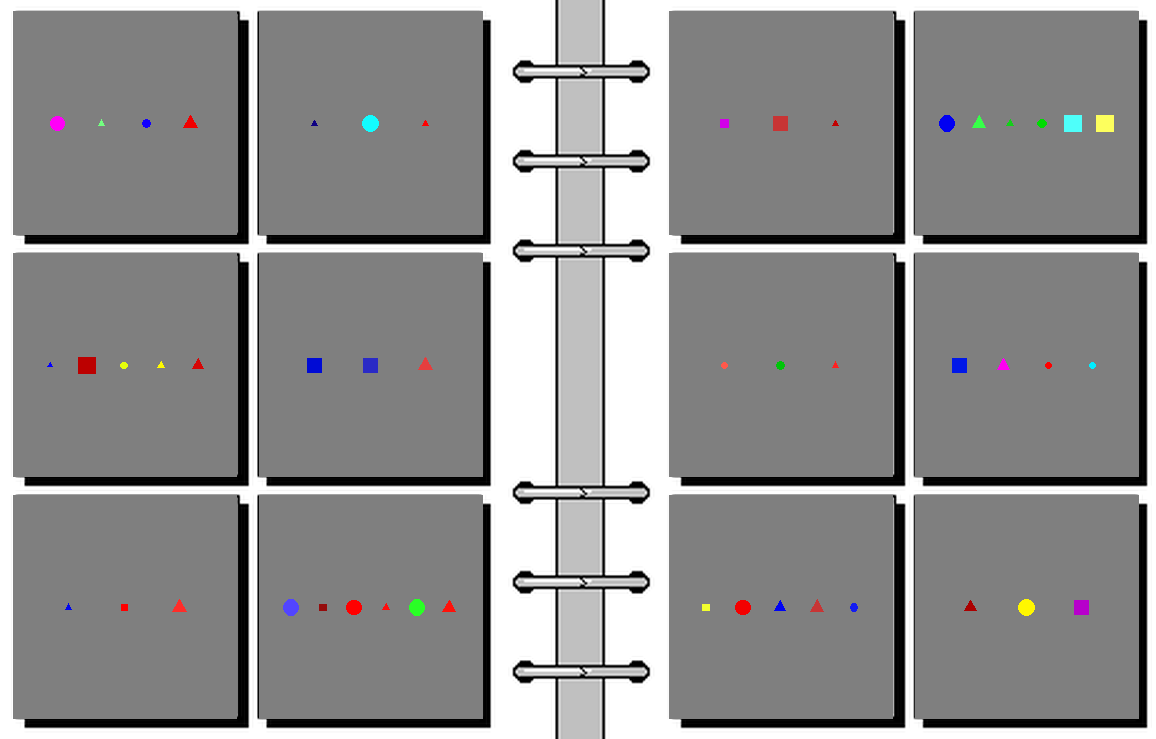
\includegraphics[width=.8\linewidth]{imgs/bongard/easy-12.png}\\
	\begin{dialogue}
		\speak{LLaVA} The Bongard Problem is a classic problem in visual reasoning, which involves determining the property that the left panels share and the property that the right panels violate. In this case, \textcolor{red}{the left panels all have three objects}, while the right panels have a different number of objects. By identifying these patterns and counting the objects, we can reason about the spatial relations and structure of the arrangement.
		%\\\direct{Did not answer.}
		%\speak{LLaVA} 
		\vspace{1em}
		\speak{MoE-LLaVA} The property that the panels on the left side of the image violate is the \textcolor{red}{color of the objects}. All the objects in the left panels are \textcolor{red}{red}, while the objects in the right panels are \textcolor{red}{green}. This creates a visual contrast between the two sets of panels, making it easier to identify the pattern. The other panels in the image do not violate any property, as they all contain objects with different shapes, colors, and sizes. The spatial relations between the objects in each panel are also consistent, with the objects being recursively displaced in a grid pattern. The logical operators used in this task are the comparison of the color of the objects in each panel, which helps to identify the pattern and solve the problem.
		%\\\direct{Did not answer.}
		%\speak{MoE-LLaVa} 
		\vspace{1em}
		\speak{InternLM-XComposer} In the panels on both sides of the image, we observe a pattern related to object placement and properties.
		
		Observations:
		
		Each panel contains atomic objects only having "small" or "large" sizes.
		The top and bottom parts of all panels mirror each other similarly.
		
		Property Under Examination on Left Side:
		
		Each panel has at least \textcolor{red}{one} small \textcolor{ForestGreen}{blue} triangle.
		Vertical symmetry: The colors are consistent vertically for any given location in each panel on the left side.
		
		Property Violated on Right Side:
		
		The vertical symmetry observed in panels on the left side is violated across the central axis. In panels on the right, various triangles appear in opposite locations compared with their counterparts' placement on the left side.
		
		Considering these observations, we infer that an important property distinguishing the left panels from the right ones relates to the spatial configuration of smaller blue triangles. \textcolor{ForestGreen}{The vertical consistency that is maintained on the left side} is violated on the right. Moreover, the spatial arrangement must directly relate to this specific property being examined.
		
		Therefore, based on logical reasoning involving object properties (color, size), spatial relations, patterns and symmetries, the central feature defining the problem relates to \textcolor{ForestGreen}{the vertical orientation and color consistency of the triangles} in each panel's vertical alignment. This is evident in the left rows but absent in the right rows of each section:
		
		Panels on the left have an identifiable property involving this consistent alignment pattern.
		Panels on the right violate this specific property.
		\\\direct{Exceeded maximum number of tokens.}
		%\\\direct{Did not answer.}
		%\speak{InternLM-XComposer} 
	\end{dialogue}
	\captionof{figure}{\textsc{KANDY-Bongard-1},  Task 12: ``There are a red triangle on the right and a blue object''}
	\label{fig:task12-bongard}
\end{tcolorbox}




\begin{tcolorbox}[breakable,enhanced jigsaw,opacityback=0,]
	\centering
	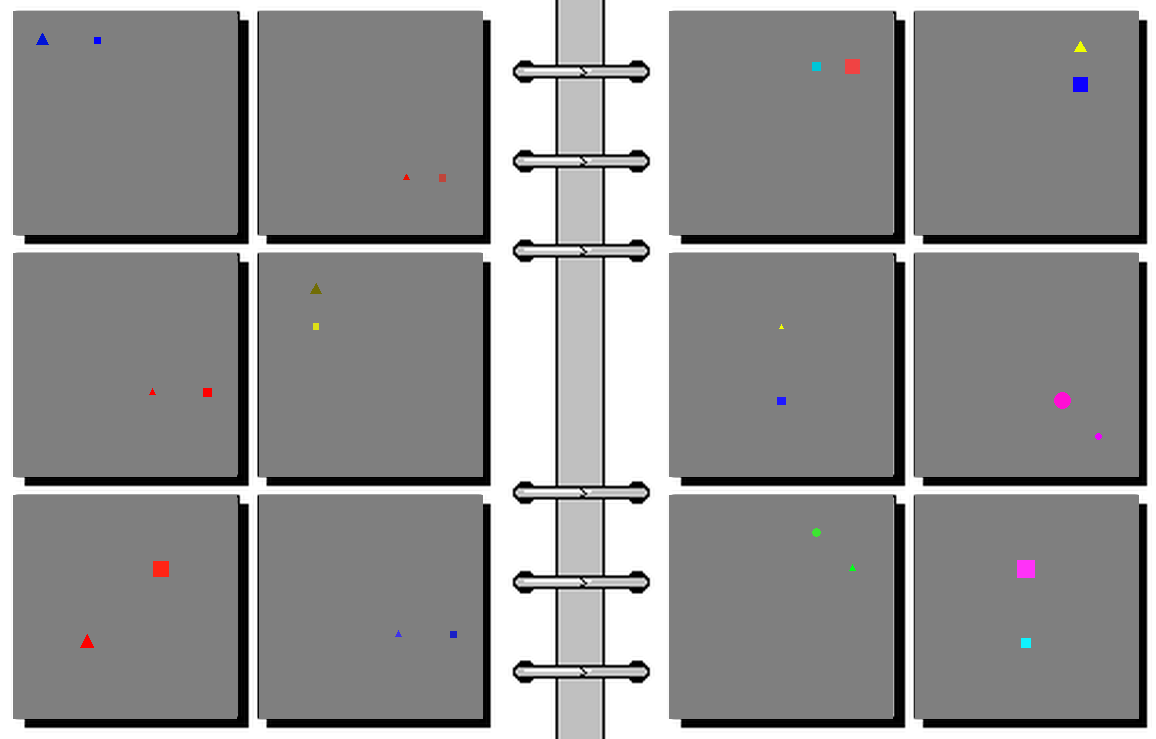
\includegraphics[width=.8\linewidth]{imgs/bongard/easy-13.png}\\
	\begin{dialogue}
		\speak{LLaVA} The image consists of twelve panels, each containing atomic objects characterized by shape, color, and size. The objects are recursively displaced vertically, horizontally, diagonally, or in a grid pattern. The panels on the left side of the image all share a single property, while the panels on the right side violate that property.
		
		The property that all panels on the left share is that the objects are arranged in a \textcolor{red}{grid pattern}. This can be observed by the alignment of the objects within each panel, creating a uniform and organized appearance. The panels on the right side, however, do not follow this pattern, which distinguishes them from the left panels.
		
		To determine the property violated by the panels on the right, one would need to analyze the arrangement of objects within each panel and compare it to the grid pattern observed in the left panels. This could involve looking for irregularities in the arrangement, such as objects not being aligned in a grid pattern or objects being displaced in a different manner than the left panels.
		%\\\direct{Did not answer.}
		%\speak{LLaVA} 
		\vspace{1em}
		\speak{MoE-LLaVA} The property that the panels on the right side of the image violate is that \textcolor{red}{they all contain the same shape and color, while the panels on the left side do not}. This creates a visual pattern that can be used to reason about the arrangement of the objects within the image.
		
		To solve this problem, one can start by identifying the shape and color of the objects in each panel. Then, by analyzing the spatial relations between the objects, one can determine the possible positions of the objects within each panel. By using logical operators such as AND, OR, and NOT, one can narrow down the possible arrangements of the objects.
		
		For example, if the objects in the left panels are triangles, and the objects in the right panels are squares, one can use the AND operator to determine that the objects in the left panels must be triangles and the objects in the right panels must be squares. Similarly, one can use the OR operator to determine that the objects in the left panels can be either red or green, while the objects in the right panels can be either blue or yellow.
		
		By using these logical operators and analyzing the spatial relations between the objects, one can reason about the arrangement of the objects within the image and determine the solution to the Bongard Problem.
		%\\\direct{Did not answer.}
		%\speak{MoE-LLaVa} 
		\vspace{1em}
		\speak{InternLM-XComposer} The objects in the image exhibit properties that \textcolor{ForestGreen}{involve their color} and spatial relationships. By systematically analyzing each panel, we can determine the pattern described.
		
		Left panels have an object that is red or blue in color (depending on which specific segment we look at).
		Each such panel also has no yellow object.
		Objects are grouped by their sizes: large and small of either color (blue or red).
		
		Left panels:
		
		\textcolor{red}{Red triangle and small blue square on a grey background.
			Red circle and small blue square on a grey background.
			Large red triangle, small red circle, and two small blue squares on a grey background}.
		
		Right panels:
		
		Yellow triangle and red circle on a grey background.
		Green circle and blue square on a grey background.
		
		The property in question is clearly related to color and spatial presence ("Objects appear with certain colors and only some panels display them"). The panels on the left side ("left of the central line") follow this logic, while the panels on the right side ("right of the central line") do not because there is a discrepancy in color consistency.
		
		In this problem, examining the symmetry and distribution of objects across different panels assists in identifying the unique property present or absent in the sets based on their arrangement, color, and combination with other elements. Understanding what causes these divisions will reveal the specific rule the panels adhere to or violate.
		%\\\direct{Did not answer.}
		%\speak{InternLM-XComposer} 
	\end{dialogue}
	\captionof{figure}{\textsc{KANDY-Bongard-1},  Task 13: ``There are a triangle and a square with the same color''}
	\label{fig:task13-bongard}
\end{tcolorbox}




\begin{tcolorbox}[breakable,enhanced jigsaw,opacityback=0,]
	\centering
	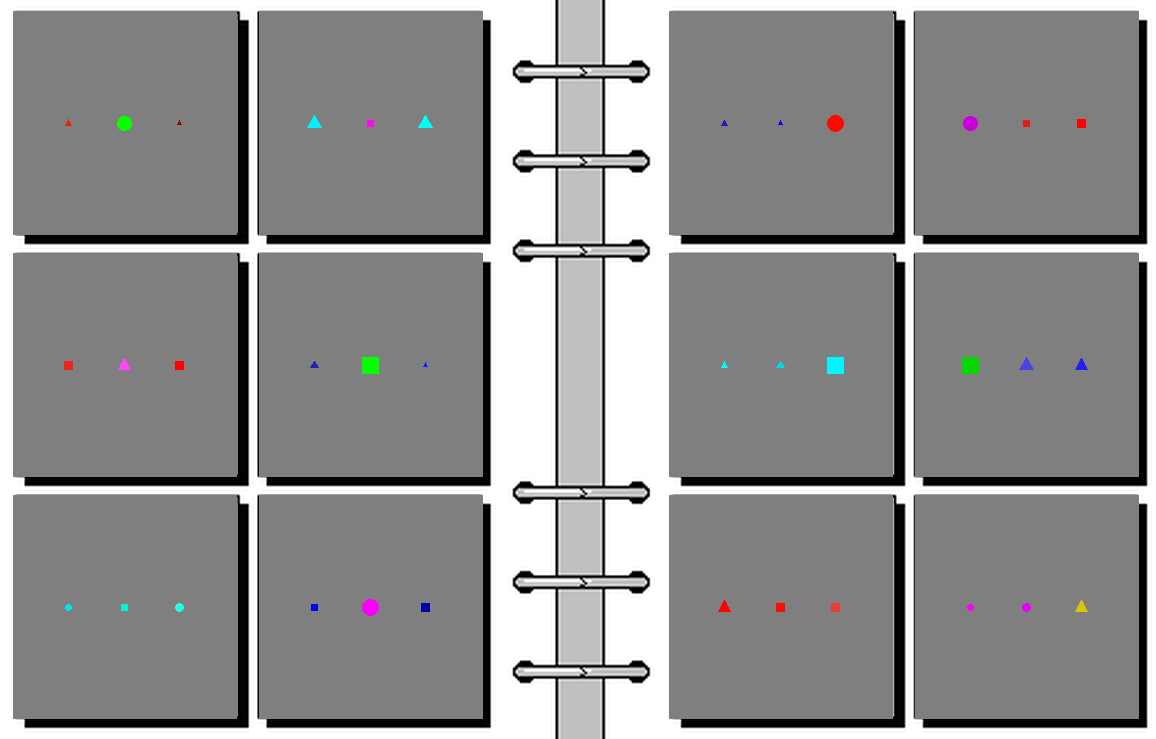
\includegraphics[width=.8\linewidth]{imgs/bongard/easy-14.png}\\
	\begin{dialogue}
		\speak{LLaVA} The image represents a Bongard Problem, which is an abstract visual reasoning task. The image consists of twelve panels, each containing atomic objects characterized by shape, color, and size. The objects are recursively displaced vertically, horizontally, diagonally, or in a grid pattern.
		
		The panels on the left side of the image all share a single property, which is that \textcolor{red}{the objects are arranged in a grid pattern}. In contrast, the panels on the right side of the image violate this property, as the objects are not arranged in a grid pattern. This difference in arrangement between the left and right panels helps to identify the property being considered in this Bongard Problem.
		%\\\direct{Did not answer.}
		%\speak{LLaVA} 
		\vspace{1em}
		\speak{MoE-LLaVA} The property that the panels on the left side of the image violate is the \textcolor{red}{color of the atomic objects}. All the panels on the left side have objects with the same color, while the panels on the right side have objects with different colors. This property violation creates a visual pattern that can be used to solve the Bongard Problem.
		
		To solve the problem, one can observe that the panels on the left side all have objects with the same color, which is a property violation. By identifying this pattern, one can deduce that the objects in the panels on the right side must have different colors. This reasoning can be further supported by the fact that the panels on the right side have objects with different colors, while the panels on the left side have objects with the same color.
		
		By recognizing the pattern and applying logical reasoning, one can successfully solve the Bongard Problem and identify the correct arrangement of the atomic objects within the panels.
		%\\\direct{Did not answer.}
		%\speak{MoE-LLaVa} 
		\vspace{1em}
		\speak{InternLM-XComposer} The property that is shared by the panels on the left side of the image and contradicted by those on the right can be deduced based on observable patterns:
		
		Object Types and Colors: Across the left panels:
		Each panel contains exactly one triangle, one large shape, and one color specific to each column.
		
		Spatial Arrangement of Colors:
		Objects with multiple colors are arranged such that at least two colors overlap vertically.
		
		Contrast in Object Arrangement: This difference doesn’t pertain to the objects but rather their arrangement or spatial positioning.
		
		The only difference detected across both sides is the \textcolor{red}{alignment of small shapes, where certain panels on the left align these elements centrally}, whereas all panels on the right do not share this exact central alignment, revealing a logical contradiction.
		
		Therefore, the observed property of the left panels which contrasts with the right panels is the central alignment of the small shapes.
		%\\\direct{Did not answer.}
		%\speak{InternLM-XComposer} 
	\end{dialogue}
	\captionof{figure}{\textsc{KANDY-Bongard-1},  Task 14: ``A palindrome of three objects''}
	\label{fig:task14-bongard}
\end{tcolorbox}




\begin{tcolorbox}[breakable,enhanced jigsaw,opacityback=0,]
	\centering
	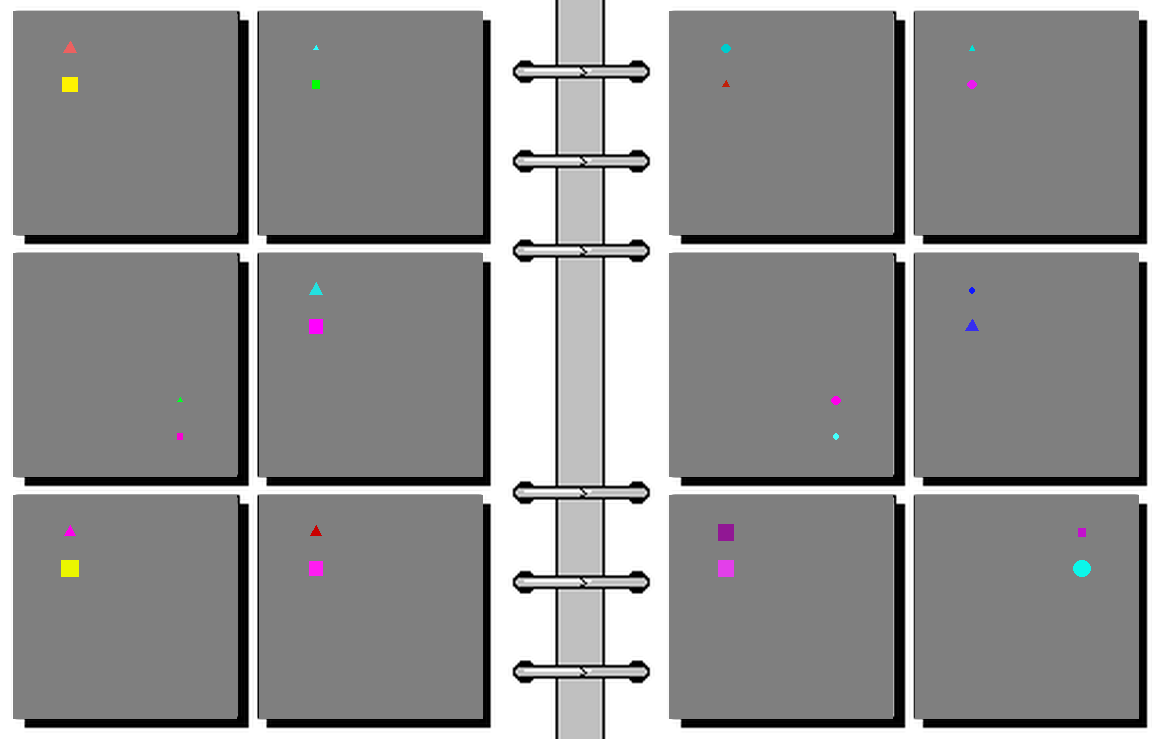
\includegraphics[width=.8\linewidth]{imgs/bongard/easy-15.png}\\
	\begin{dialogue}
		\speak{LLaVA} The image consists of twelve panels, each containing atomic objects characterized by shape, color, and size. The objects are recursively displaced vertically, horizontally, diagonally, or in a grid pattern. The panels on the left side of the image all share a single property, while the panels on the right side violate that property.
		
		The property that the panels on the left share is that \textcolor{red}{all the objects within each panel are of the same color}. This can be observed by looking at the panels and noticing that all the objects within each panel have the same color. The panels on the right side, however, violate this property by having objects with different colors within each panel. This can be observed by looking at the panels and noticing that some objects have different colors within each panel.
		%\\\direct{Did not answer.}
		%\speak{LLaVA} 
		\vspace{1em}
		\speak{MoE-LLaVA} The property that the panels on the left side of the image violate is the color of the atomic objects. All the panels on the left side have \textcolor{red}{objects with the same color}, while the panels on the right side have objects with different colors. This property violation can be used to create a visual reasoning task that requires identifying the pattern and reasoning about the spatial relationships between the objects in each panel. The task can be solved by analyzing the patterns and \textcolor{red}{counting the number of objects with the same color in each panel}, and then comparing the results to the expected pattern.
		%\\\direct{Did not answer.}
		%\speak{MoE-LLaVa} 
		\vspace{1em}
		\speak{InternLM-XComposer} In analyzing the Bongard Problem, several features and properties should be noted across the twelve panels.
		
		Spatial Relations:
		Panels on the left demonstrate a \textcolor{ForestGreen}{consistent arrangement of objects within each panel} that includes \textcolor{ForestGreen}{either all small objects or all large objects without any mixed sizes}.
		Panels on the right display an inconsistency in object size.
		
		Color Patterns:
		\textcolor{red}{All panels (left and right) contain only specific colors (red, green, blue, cyan, magenta, yellow), likely indicating no multiple colors per panel}.
		
		Object Shape and Size:
		Panels have different orientations in which \textcolor{ForestGreen}{the shapes follow a consistent pattern throughout the left side}, while the right side shows a mix with varying shape sizes.
		
		Symmetry and Pattern Recognition:
		Symmetry is present in some panels within left category where there are \textcolor{ForestGreen}{recursive patterns of same-color}, \textcolor{red}{possibly in concentric circles}.
		
		Based on this reasoning:
		
		The property shared by the panels on the left would require the characteristic of \textcolor{ForestGreen}{consistent color and size distribution between the shapes, specifically adhering to a pattern}.
		On the right, this consistency of color and size is broken.
		
		Thus, the defining feature of the left panels is the consistency in color and shape sizes while disregarding emptiness, spatial order, and symmetrical relationships observed uniformly across the left half.
		%\\\direct{Did not answer.}
		%\speak{InternLM-XComposer} 
	\end{dialogue}
	\captionof{figure}{\textsc{KANDY-Bongard-1},  Task 15: ``A house (triangle above a square)''}
	\label{fig:task15-bongard}
\end{tcolorbox}




\begin{tcolorbox}[breakable,enhanced jigsaw,opacityback=0,]
	\centering
	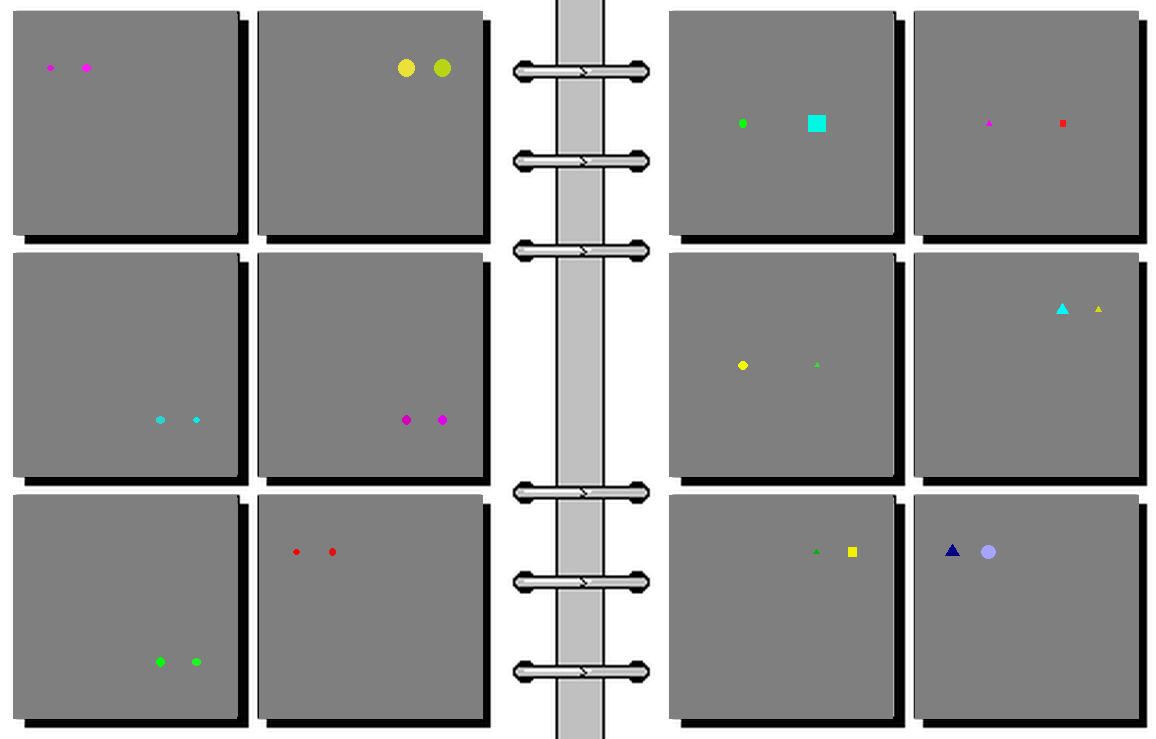
\includegraphics[width=.8\linewidth]{imgs/bongard/easy-16.png}\\
	\begin{dialogue}
		\speak{LLaVA} The image consists of twelve panels, each containing atomic objects characterized by shape, color, and size. The objects are recursively displaced vertically, horizontally, diagonally, or in a grid pattern. The panels on the left side of the image all share a single property, while the panels on the right side violate that property.
		
		The property that the panels on the left share is that \textcolor{ForestGreen}{all the objects within each panel are of the same color}. This can be observed by looking at the colors of the objects in each panel. The panels on the right side, however, violate this property by having objects of different colors within the same panel.
		
		To identify the property, one can look at the colors of the objects in each panel and compare them to the colors of the objects in the other panels. This will help to identify the property that the panels on the left share and the property that the panels on the right violate.
		%\\\direct{Did not answer.}
		%\speak{LLaVA} 
		\vspace{1em}
		\speak{MoE-LLaVA} The property that is violated in the panels on the right side of the image is the color of the objects. \textcolor{ForestGreen}{The panels on the left all share the same color}, while the panels on the right have different colors. This property violation creates a visual challenge for the viewer to identify the patterns and relationships between the objects within each panel. The viewer must use their visual reasoning skills to determine the correct arrangement of the objects based on the given information.
		%\\\direct{Did not answer.}
		%\speak{MoE-LLaVa} 
		\vspace{1em}
		\speak{InternLM-XComposer} In analyzing the provided image, identify the repeating pattern in the panels on the left side and contrast it with the violations seen in the panels on the right.
		
		Here's the analysis:
		
		Objects by Shape, Size, Color and Position: Look for recurring shapes, colors, or positions in the consistent panels.
		
		Total Count: Count total objects per panel, ensuring both object type and color are factored in.
		
		Spacial Distribution: Examine if there is any specific spacial relation that consistent panels may have (e.g., alignment).
		
		Symmetry: Analyzing symmetrical properties in consistent panels can guide reasoning.
		
		Pattern in Object Size: Observe if there is a common pattern of large/small objects between consistent and inconsistant panels.
		
		Pattern in Object Color: Check for repeated color patterns or unique coloring in alternating grids.
		
		Specific Color Patterns or Distribution: Some specific panels follow a single color, perhaps consistently used as a backdrop or for a certain position.
		
		Count or Position Pattern: Consistency might lie in the number or vertical position of objects.
		
		Upon examining the left and right panels:
		
		On the left, \textcolor{red}{2 green triangles and 2 cyan squares repeat across four panels}.
		On the right, this repetition is violated; the objects differ in terms of colors (left includes no blue elements) and their positions show irregularity.
		
		Thus, deduce from these observations that consistency involves \textcolor{ForestGreen}{equal-sized objects} (large and small), while violations involve variations among blue-colored circles, green squares, or differing vertical alignments of objects.
		
		Based on this reasoning, it appears that all consistent panels contain a single recurring object property. The property is that each panel contains an equal number and color of items that fall within a certain range. Without more details on the specifics required to solve entirely, the general pattern indicates object equivalence across certain categorical parameters, either geometrically, spatially, or colorically.
		%\\\direct{Did not answer.}
		%\speak{InternLM-XComposer} 
	\end{dialogue}
	\captionof{figure}{\textsc{KANDY-Bongard-1},  Task 16: ``A car (two side-by-side circles with the same color)''}
	\label{fig:task16-bongard}
\end{tcolorbox}




\begin{tcolorbox}[breakable,enhanced jigsaw,opacityback=0,]
	\centering
	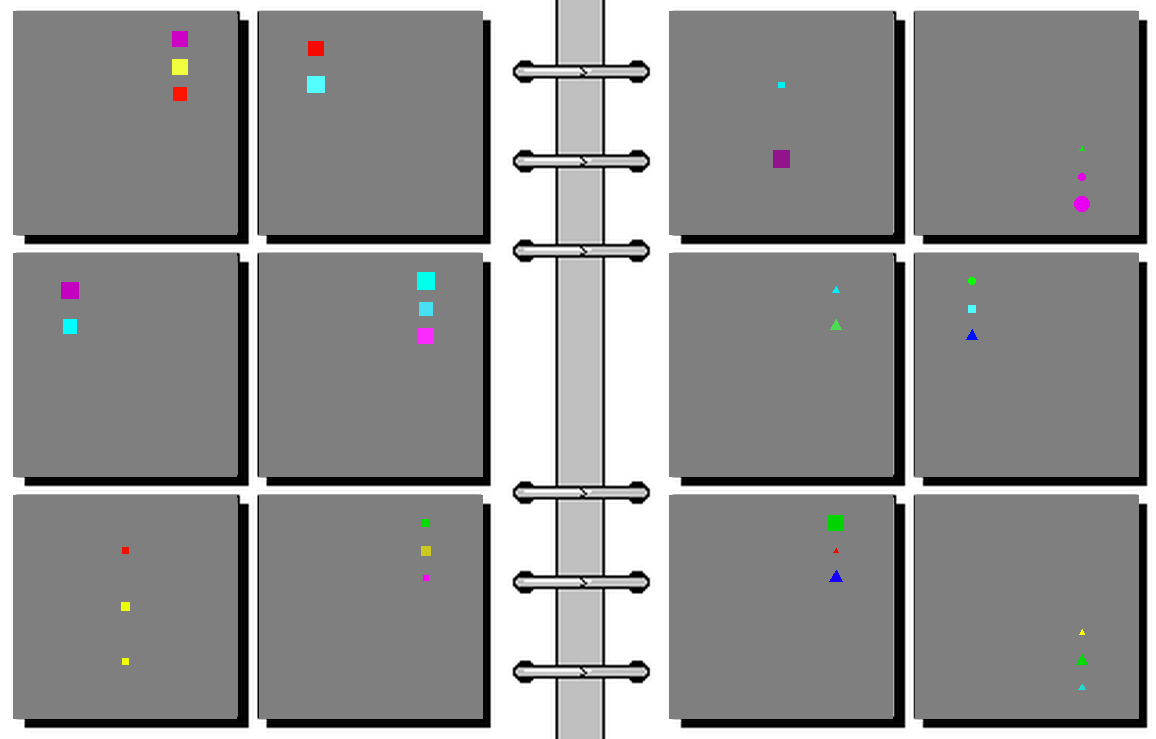
\includegraphics[width=.8\linewidth]{imgs/bongard/easy-17.png}\\
	\begin{dialogue}
		\speak{LLaVA} The image features twelve panels, each containing atomic objects characterized by shape, color, and size. The objects are recursively displaced vertically, horizontally, diagonally, or in a grid pattern. The panels on the left side of the image all share a single property, while the panels on the right side violate that property.
		
		The property that the left panels share is that \textcolor{red}{all the objects within each panel are of the same color}. This can be observed by looking at the color distribution across the panels. The panels on the right side, however, have objects with different colors, which violates the property shared by the left panels.
		%\\\direct{Did not answer.}
		%\speak{LLaVA} 
		\vspace{1em}
		\speak{MoE-LLaVA} The property that the panels on the left side of the image share is that \textcolor{ForestGreen}{they all contain only one type of object, which is a square}. The other panels on the right side of the image violate this property by containing a variety of objects, including triangles, circles, and other shapes. This property can be used to reason about the spatial relations between the objects within each panel and to identify patterns and symmetries in the arrangement of the objects. Additionally, the logical operator "not" can be used to identify the panels that do not share the same property as the others.
		%\\\direct{Did not answer.}
		%\speak{MoE-LLaVa} 
		\vspace{1em}
		\speak{InternLM-XComposer} The property that characterizes the panels on the left side of the image is \textcolor{red}{"there is a combination of two colors, with at least one triangle"}. Here are the details:
		
		Object properties and colors:
		Panels in the left side each have exactly 2 or more colors: either yellow-red, magenta-cyan, and so on.
		
		Property violation in panels on the right side:
		Each panel on the right side has three different colors but does not contain triangles, thus violating the property.
		
		Ignoring empty panels:
		Some panels may lack objects, which does not matter for this property.
		
		Counting and symmetry:
		Each group of panels (left) contains an equal number from each category based on their color combinations, but these are usually mixed and distributed in terms of spatial relation.
		
		Spatial relations and patterns:
		Panels are arranged symmetrically around the central spine (axis of symmetry).
		The triangles are either at the top or bottom half while squares are on the outside in even arrangement.
		
		Logical operators:
		The panels seem to be divided into groups where each panel meets four other panels, ensuring that the patterns are consistent across all such subsets.
		
		Additional features that may help:
		All the unique color combinations (red-yellow, magenta-cyan) maintain spatial consistency.
		
		Based on these observations, we conclude that the property of interest ensures all panels on either side of the central spine have a consistent usage of object properties relative to shapes and colors, implying spatial symmetry (regular distribution).
		%\\\direct{Did not answer.}
		%\speak{InternLM-XComposer} 
	\end{dialogue}
	\captionof{figure}{\textsc{KANDY-Bongard-1},  Task 17: ``A tower (two or more squares of the same size  stacked vertically)''}
	\label{fig:task17-bongard}
\end{tcolorbox}




\begin{tcolorbox}[breakable,enhanced jigsaw,opacityback=0,]
	\centering
	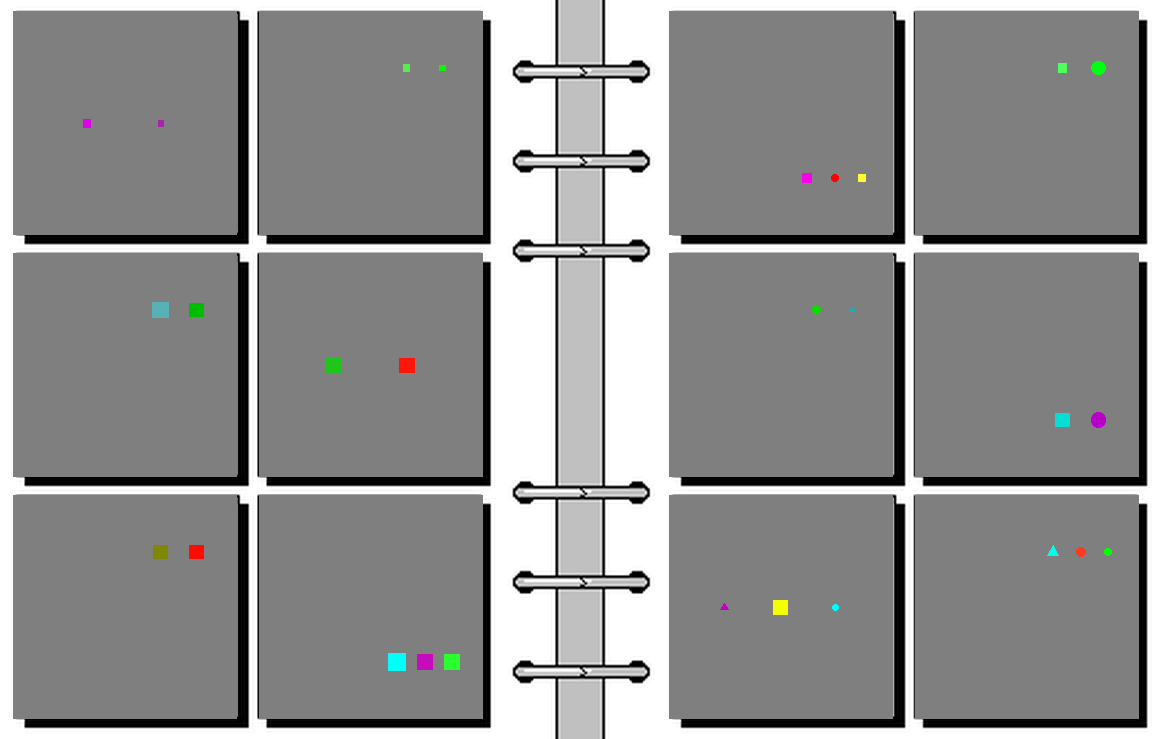
\includegraphics[width=.8\linewidth]{imgs/bongard/easy-18.png}\\
	\begin{dialogue}
		\speak{LLaVA} The image represents a Bongard Problem, which is an abstract visual reasoning task. The image consists of twelve panels, each containing atomic objects characterized by shape, color, and size. The objects are recursively displaced vertically, horizontally, diagonally, or in a grid pattern.
		
		The panels on the left side of the image all share a single property, which is that \textcolor{red}{the objects are arranged in a grid pattern}. On the other hand, the panels on the right side of the image violate this property, as the objects are not arranged in a grid pattern. This difference in arrangement between the left and right panels helps to identify the property that the panels share.
		%\\\direct{Did not answer.}
		%\speak{LLaVA} 
		\vspace{1em}
		\speak{MoE-LLaVA} The image represents an abstract visual reasoning task, known as a Bongard Problem, and it is composed of twelve panels. Each panel contains atomic objects characterized by shape ("triangle", "square", "circle"), color ("red", "green", "blue", "cyan", "magenta", "yellow") and size ("small", "large"). Atomic objects are recursively displaced vertically, horizontally, diagonally or in a grid pattern. Objects within each panel can be characterized by some property. The panels on the left part of the image all share a single property. Conversely, the panels on the right side violate that property. Please describe the property, ignoring empty panels, if any. You are allowed to reason in terms of: object properties, spatial relations, patterns, counting, symmetries and logical operators. Enumerate any feature which may help.
		
		The property that the panels on the right side of the image violate is the \textcolor{red}{color of the atomic objects}. In the left panels, all the objects have the same color, while in the right panels, the objects have different colors. This property violation is a key aspect of the Bongard Problem, which is an abstract visual reasoning task that requires the ability to identify patterns and relationships between objects.
		%\\\direct{Did not answer.}
		%\speak{MoE-LLaVa} 
		\vspace{1em}
		\speak{InternLM-XComposer} Upon inspecting the image, one can identify that the object of interest for solving this problem is to determine if there are \textcolor{red}{color matches horizontally between each pair of panels}.
		
		Panels on the left side: Each panel displays a \textcolor{red}{triangle and a square} with matching colors horizontally.
		Panels on the right side: The two middle panels violate this property; they have mismatched horizontal color pairs or no horizontal color pairs at all.
		
		Therefore, the property we are identifying is that in exactly half of the panels, each horizontal alignment contains at least two objects with matching colors. In contrast, three panels on the right side do not meet this criterion.
		%\\\direct{Did not answer.}
		%\speak{InternLM-XComposer} 
	\end{dialogue}
	\captionof{figure}{\textsc{KANDY-Bongard-1},  Task 18: ``A wagon (two or more squares of the same size side by side)''}
	\label{fig:task18-bongard}
\end{tcolorbox}




\begin{tcolorbox}[breakable,enhanced jigsaw,opacityback=0,]
	\centering
	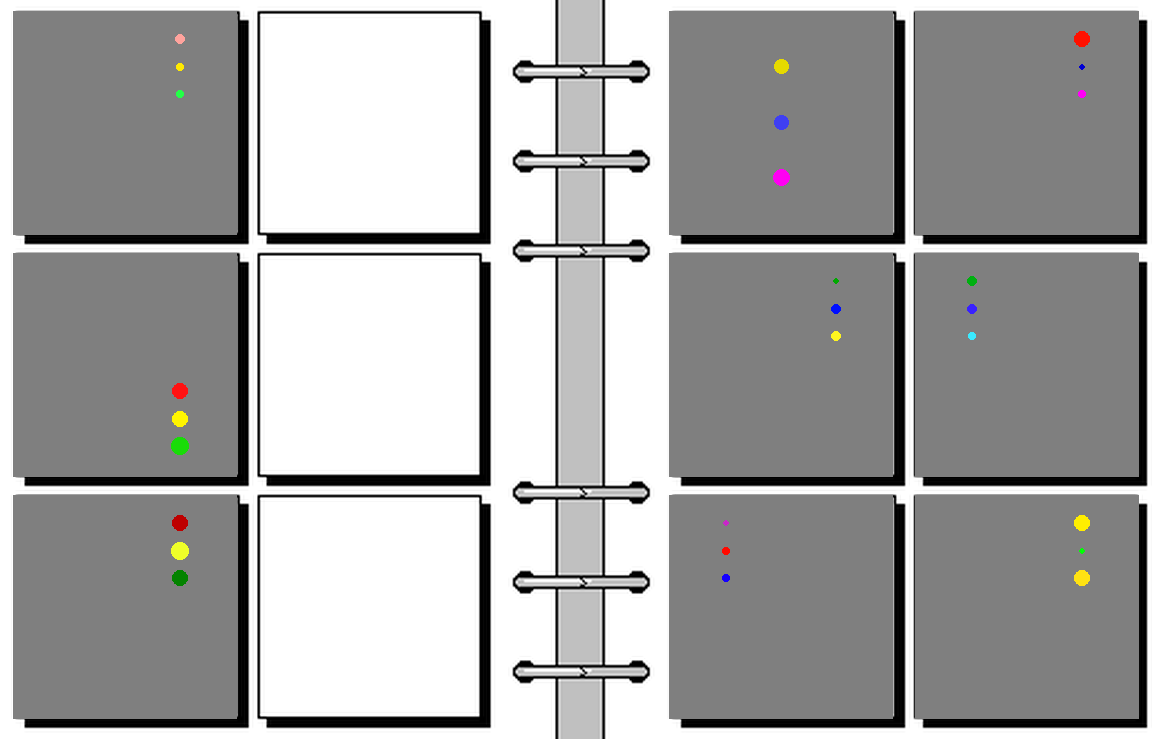
\includegraphics[width=.8\linewidth]{imgs/bongard/easy-19.png}\\
	\begin{dialogue}
		\speak{LLaVA} The image features twelve panels, each containing atomic objects characterized by shape, color, and size. The objects are recursively displaced vertically, horizontally, diagonally, or in a grid pattern. The panels on the left side of the image all share a single property, while the panels on the right side violate that property.
		
		The property that the left panels share is that all the objects within each panel are of the \textcolor{red}{same color}. This can be observed by looking at the color distribution in each panel. The panels on the right side, however, have objects with different colors, breaking the uniformity of color within each panel. This difference in color distribution distinguishes the left and right panels.
		%\\\direct{Did not answer.}
		%\speak{LLaVA} 
		\vspace{1em}
		\speak{MoE-LLaVA} The property that the panels on the left side of the image violate is that \textcolor{ForestGreen}{they all have the same shape, color, and size}. This is a violation of the rule that objects within each panel should have different properties. The panels on the right side of the image, however, follow the rule by having different shapes, colors, and sizes. This property can be identified by observing the arrangement of the panels and the objects within them, and by comparing the properties of the objects in each panel.
		%\\\direct{Did not answer.}
		%\speak{MoE-LLaVa} 
		\vspace{1em}
		\speak{InternLM-XComposer} In the given image with twelve panels, we observe that the patterns in both the left and right sides differ.
		
		\textcolor{ForestGreen}{Red dot}: The red dot appears only vertically on the right side.
		Blue dot: The blue dot appears only diagonally at the top right corner on the right side.
		
		Comparing these elements to the left panels:
		
		The left panels display a pattern where a certain object (either an atomic object) is consistently aligned horizontally.
		In contrast, none of this pattern of alignment is observed in the right panels.
		
		Thus, considering all panel components as well as object properties, spatial relations, and logical operators:
		
		Objects are arranged both vertically and horizontally, but not the same as across both parts of the panels.
		The panels show different arrangement patterns on both sides.
		Left: Horizontal alignment
		Right: Vertical alignment
		
		Based on this reasoning and observing the commonalities:
		The specific feature which helps identify the property being violated or observed in the respective panels is the horizontal alignment present in the left panels versus the vertical alignment in the right panels. Hence, the property that could be defined would likely relate to the direction of alignment.
		
		Therefore, the correct enumeration based on the given parameters is:
		The panels on the left side feature horizontal alignment of objects within them. Conversely, the panels on the right side have objects that are typically aligned vertically—therefore, violating the horizontal alignment property.
		%\\\direct{Did not answer.}
		%\speak{InternLM-XComposer} 
	\end{dialogue}
	\captionof{figure}{\textsc{KANDY-Bongard-1},  Task 19: ``A traffic light (a red, a yellow and a green circle of the same size vertically stacked)''}
	\label{fig:task19-bongard}
\end{tcolorbox}
